% ****************************************************************************************
% *****************           PROPABILIDAD Y ESTADISTICA      ****************************
% ****************************************************************************************


% =======================================================
% =======         HEADER FOR DOCUMENT        ============
% =======================================================
    
    % *********   HEADERS AND FOOTERS ********
    \def\ProjectAuthorLink{https://github.com/SoyOscarRH}           %Just to keep it in line
    \def\ProjectNameLink{\ProjectAuthorLink/LibroProbabilidad}      %Link to Proyect

    % *********   DOCUMENT ITSELF   **************
    \documentclass[12pt, fleqn]{report}                             %Type of docuemtn and size of font and left eq
    \usepackage[spanish]{babel}                                     %Please use spanish
    \usepackage[utf8]{inputenc}                                     %Please use spanish - UFT
    \usepackage[margin = 1.2in]{geometry}                           %Margins and Geometry pacakge
    \usepackage{ifthen}                                             %Allow simple programming
    \usepackage{hyperref}                                           %Create MetaData for a PDF and LINKS!
    \usepackage{pdfpages}                                           %Create MetaData for a PDF and LINKS!
    \hypersetup{pageanchor = false}                                 %Solve 'double page 1' warnings in build
    \setlength{\parindent}{0pt}                                     %Eliminate ugly indentation
    \author{Oscar Andrés Rosas}                                     %Who I am

    % *********   LANGUAJE    *****************
    \usepackage[T1]{fontenc}                                        %Please use spanish
    \usepackage{textcmds}                                           %Allow us to use quoutes
    \usepackage{changepage}                                         %Allow us to use identate paragraphs
    \usepackage{anyfontsize}                                        %All the sizes

    % *********   MATH AND HIS STYLE  *********
    \usepackage{ntheorem, amsmath, amssymb, amsfonts}               %All fucking math, I want all!
    \usepackage{mathrsfs, mathtools, empheq}                        %All fucking math, I want all!
    \usepackage{cancel}                                             %Negate symbol
    \usepackage{centernot}                                          %Allow me to negate a symbol
    \decimalpoint                                                   %Use decimal point

    % *********   GRAPHICS AND IMAGES *********
    \usepackage{graphicx}                                           %Allow to create graphics
    \usepackage{float}                                              %For images
    \usepackage{wrapfig}                                            %Allow to create images
    \graphicspath{ {Graphics/} }                                    %Where are the images :D

    % *********   LISTS AND TABLES ***********
    \usepackage{listings, listingsutf8}                             %We will be using code here
    \usepackage[inline]{enumitem}                                   %We will need to enumarate
    \usepackage{tasks}                                              %Horizontal lists
    \usepackage{longtable}                                          %Lets make tables awesome
    \usepackage{booktabs}                                           %Lets make tables awesome
    \usepackage{tabularx}                                           %Lets make tables awesome
    \usepackage{multirow}                                           %Lets make tables awesome
    \usepackage{multicol}                                           %Create multicolumns

    % *********   HEADERS AND FOOTERS ********
    \usepackage{fancyhdr}                                           %Lets make awesome headers/footers
    \pagestyle{fancy}                                               %Lets make awesome headers/footers
    \setlength{\headheight}{16pt}                                   %Top line
    \setlength{\parskip}{0.5em}                                     %Top line
    \renewcommand{\footrulewidth}{0.5pt}                            %Bottom line

    \lhead {                                                        %Left Header
        \hyperlink{chapter.\arabic{chapter}}                        %Make a link to the current chapter
        {\normalsize{\textsc{\nouppercase{\leftmark}}}}             %And fot it put the name
    }

    \rhead {                                                        %Right Header
        \hyperlink{section.\arabic{chapter}.\arabic{section}}       %Make a link to the current chapter
            {\footnotesize{\textsc{\nouppercase{\rightmark}}}}      %And fot it put the name
    }

    \rfoot{\textsc{\small{\hyperref[sec:Index]{Ve al Índice}}}}     %This will always be a footer  

    \fancyfoot[L]{                                                  %Algoritm for a changing footer
        \ifthenelse{\isodd{\value{page}}}                           %IF ODD PAGE:
            {\href{https://compilandoconocimiento.com/nosotros/}    %DO THIS:
                {\footnotesize                                      %Send the page
                    {\textsc{Oscar Andrés Rosas}}}}                 %Send the page
            {\href{https://compilandoconocimiento.com}              %ELSE DO THIS: 
                {\footnotesize                                      %Send the author
                    {\textsc{Compilando Conocimiento}}}}            %Send the author
    }
    
    
    
% =======================================================
% ===================   COMMANDS    =====================
% =======================================================

    % =========================================
    % =======   NEW ENVIRONMENTS   ============
    % =========================================
    \newenvironment{Indentation}[1][0.75em]                         %Use: \begin{Inde...}[Num]...\end{Inde...}
        {\begin{adjustwidth}{#1}{}}                                 %If you dont put nothing i will use 0.75 em
        {\end{adjustwidth}}                                         %This indentate a paragraph
    \newenvironment{SmallIndentation}[1][0.75em]                    %Use: The same that we upper one, just 
        {\begin{adjustwidth}{#1}{}\begin{footnotesize}}             %footnotesize size of letter by default
        {\end{footnotesize}\end{adjustwidth}}                       %that's it

    \newenvironment{MultiLineEquation}[1]                           %Use: To create MultiLine equations
        {\begin{equation}\begin{alignedat}{#1}}                     %Use: \begin{Multi..}{Num. de Columnas}
        {\end{alignedat}\end{equation}}                             %And.. that's it!
    \newenvironment{MultiLineEquation*}[1]                          %Use: To create MultiLine equations
        {\begin{equation*}\begin{alignedat}{#1}}                    %Use: \begin{Multi..}{Num. de Columnas}
        {\end{alignedat}\end{equation*}}                            %And.. that's it!
    

    % =========================================
    % == GENERAL TEXT & SYMBOLS ENVIRONMENTS ==
    % =========================================
    
    % =====  TEXT  ======================
    \newcommand \Quote {\qq}                                        %Use: \Quote to use quotes
    \newcommand \Over {\overline}                                   %Use: \Bar to use just for short
    \newcommand \ForceNewLine {$\Space$\\}                          %Use it in theorems for example

    % =====  SPACES  ====================
    \DeclareMathOperator \Space {\quad}                             %Use: \Space for a cool mega space
    \DeclareMathOperator \MegaSpace {\quad \quad}                   %Use: \MegaSpace for a cool mega mega space
    \DeclareMathOperator \MiniSpace {\;}                            %Use: \Space for a cool mini space
    
    % =====  MATH TEXT  =================
    \newcommand \Such {\MiniSpace | \MiniSpace}                     %Use: \Such like in sets
    \newcommand \Also {\MiniSpace \text{y} \MiniSpace}              %Use: \Also so it's look cool
    \newcommand \Remember[1]{\Space\text{\scriptsize{#1}}}          %Use: \Remember so it's look cool
    
    % =====  THEOREMS  ==================
    \newtheorem{Theorem}{Teorema}[section]                          %Use: \begin{Theorem}[Name]\label{Nombre}...
    \newtheorem{Corollary}{Colorario}[Theorem]                      %Use: \begin{Corollary}[Name]\label{Nombre}...
    \newtheorem{Lemma}[Theorem]{Lemma}                              %Use: \begin{Lemma}[Name]\label{Nombre}...
    \newtheorem{Definition}{Definición}[section]                    %Use: \begin{Definition}[Name]\label{Nombre}...
    \theoremstyle{break}                                            %THEOREMS START 1 SPACE AFTER

    % =====  LOGIC  =====================
    \newcommand \lIff {\leftrightarrow}                             %Use: \lIff for logic iff
    \newcommand \lEqual {\MiniSpace \Leftrightarrow \MiniSpace}     %Use: \lEqual for a logic double arrow
    \newcommand \lInfire {\MiniSpace \Rightarrow \MiniSpace}        %Use: \lInfire for a logic infire
    \newcommand \lLongTo {\longrightarrow}                          %Use: \lLongTo for a long arrow

    % =====  FAMOUS SETS  ===============
    \DeclareMathOperator \Naturals     {\mathbb{N}}                 %Use: \Naturals por Notation
    \DeclareMathOperator \Primes       {\mathbb{P}}                 %Use: \Primes por Notation
    \DeclareMathOperator \Integers     {\mathbb{Z}}                 %Use: \Integers por Notation
    \DeclareMathOperator \Racionals    {\mathbb{Q}}                 %Use: \Racionals por Notation
    \DeclareMathOperator \Reals        {\mathbb{R}}                 %Use: \Reals por Notation
    \DeclareMathOperator \Complexs     {\mathbb{C}}                 %Use: \Complex por Notation
    \DeclareMathOperator \GenericField {\mathbb{F}}                 %Use: \GenericField por Notation
    \DeclareMathOperator \VectorSet    {\mathbb{V}}                 %Use: \VectorSet por Notation
    \DeclareMathOperator \SubVectorSet {\mathbb{W}}                 %Use: \SubVectorSet por Notation
    \DeclareMathOperator \Polynomials  {\mathbb{P}}                 %Use: \Polynomials por Notation

    % =====  CONTAINERS   ===============
    \newcommand{\Set}[1]{\left\{ \; #1 \; \right\}}                 %Use: \Set {Info} for INTELLIGENT space 
    \newcommand{\bigSet}[1]{\big\{ \; #1 \; \big\}}                 %Use: \bigSet  {Info} for space 
    \newcommand{\BigSet}[1]{\Big\{ \; #1 \; \Big\}}                 %Use: \BigSet  {Info} for space 
    \newcommand{\biggSet}[1]{\bigg\{ \; #1 \; \bigg\}}              %Use: \biggSet {Info} for space 
    \newcommand{\BiggSet}[1]{\Bigg\{ \; #1 \; \Bigg\}}              %Use: \BiggSet {Info} for space 
    
    \newcommand{\Brackets}[1]{\left[ #1 \right]}                    %Use: \Brackets {Info} for INTELLIGENT space
    \newcommand{\bigBrackets}[1]{\big[ \; #1 \; \big]}              %Use: \bigBrackets  {Info} for space 
    \newcommand{\BigBrackets}[1]{\Big[ \; #1 \; \Big]}              %Use: \BigBrackets  {Info} for space 
    \newcommand{\biggBrackets}[1]{\bigg[ \; #1 \; \bigg]}           %Use: \biggBrackets {Info} for space 
    \newcommand{\BiggBrackets}[1]{\Bigg[ \; #1 \; \Bigg]}           %Use: \BiggBrackets {Info} for space 
    
    \newcommand{\Wrap}[1]{\left( #1 \right)}                        %Use: \Wrap {Info} for INTELLIGENT space
    \newcommand{\bigWrap}[1]{\big( \; #1 \; \big)}                  %Use: \bigBrackets  {Info} for space 
    \newcommand{\BigWrap}[1]{\Big( \; #1 \; \Big)}                  %Use: \BigBrackets  {Info} for space 
    \newcommand{\biggWrap}[1]{\bigg( \; #1 \; \bigg)}               %Use: \biggBrackets {Info} for space 
    \newcommand{\BiggWrap}[1]{\Bigg( \; #1 \; \Bigg)}               %Use: \BiggBrackets {Info} for space 

    % =====  BETTERS MATH COMMANDS   =====
    \newcommand{\pfrac}[2]{\Wrap{\dfrac{#1}{#2}}}                   %Use: Put fractions in parentesis

    % =========================================
    % ====   LINEAL ALGEBRA & VECTORS    ======
    % =========================================

    % ===== UNIT VECTORS  ================
    \newcommand{\hati} {\hat{\imath}}                               %Use: \hati for unit vector    
    \newcommand{\hatj} {\hat{\jmath}}                               %Use: \hatj for unit vector    
    \newcommand{\hatk} {\hat{k}}                                    %Use: \hatk for unit vector

    % ===== MAGNITUDE  ===================
    \newcommand{\abs}[1]{\left\lvert #1 \right\lvert}               %Use: \abs{expression} for |x|
    \newcommand{\Abs}[1]{\left\lVert #1 \right\lVert}               %Use: \Abs{expression} for ||x||
    \newcommand{\Mag}[1]{\left| #1 \right|}                         %Use: \Mag {Info} 
    
    \DeclareMathOperator \LinealTransformation {\mathcal{T}}        %Use: \LinealTransformation for a cool T
    \newcommand{\bVec}[1]{\mathbf{#1}}                              %Use for bold type of vector
    \newcommand{\lVec}[1]{\overrightarrow{#1}}                      %Use for a long arrow over a vector
    \newcommand{\uVec}[1]{\mathbf{\hat{#1}}}                        %Use: Unitary Vector Example: $\uVec{i}

    % ===== ALL FOR DOT PRODUCT  =========
    \makeatletter                                                   %WTF! IS THIS
    \newcommand*\dotP{\mathpalette\dotP@{.5}}                       %Use: \dotP for dot product
    \newcommand*\dotP@[2] {\mathbin {                               %WTF! IS THIS            
        \vcenter{\hbox{\scalebox{#2}{$\m@th#1\bullet$}}}}           %WTF! IS THIS
    }                                                               %WTF! IS THIS
    \makeatother                                                    %WTF! IS THIS

    % === WRAPPERS FOR COLUMN VECTOR ===
    \newcommand{\pVector}[1]                                        %Use: \pVector {Matrix Notation} use parentesis
        { \ensuremath{\begin{pmatrix}#1\end{pmatrix}} }             %Example: \pVector{a\\b\\c} or \pVector{a&b&c} 
    \newcommand{\lVector}[1]                                        %Use: \lVector {Matrix Notation} use a abs 
        { \ensuremath{\begin{vmatrix}#1\end{vmatrix}} }             %Example: \lVector{a\\b\\c} or \lVector{a&b&c} 
    \newcommand{\bVector}[1]                                        %Use: \bVector {Matrix Notation} use a brackets 
        { \ensuremath{\begin{bmatrix}#1\end{bmatrix}} }             %Example: \bVector{a\\b\\c} or \bVector{a&b&c} 
    \newcommand{\Vector}[1]                                         %Use: \Vector {Matrix Notation} no parentesis
        { \ensuremath{\begin{matrix}#1\end{matrix}} }               %Example: \Vector{a\\b\\c} or \Vector{a&b&c}

    % === MAKE MATRIX BETTER  =========
    \makeatletter                                                   %Example: \begin{matrix}[cc|c]
    \renewcommand*\env@matrix[1][*\c@MaxMatrixCols c] {             %WTF! IS THIS
        \hskip -\arraycolsep                                        %WTF! IS THIS
        \let\@ifnextchar\new@ifnextchar                             %WTF! IS THIS
        \array{#1}                                                  %WTF! IS THIS
    }                                                               %WTF! IS THIS
    \makeatother                                                    %WTF! IS THIS

    % =========================================
    % =======   FAMOUS FUNCTIONS   ============
    % =========================================

    % == TRIGONOMETRIC FUNCTIONS  ====
    \newcommand{\Cos}[1] {\cos\Wrap{#1}}                            %Simple wrappers
    \newcommand{\Sin}[1] {\sin\Wrap{#1}}                            %Simple wrappers
    \newcommand{\Tan}[1] {tan\Wrap{#1}}                             %Simple wrappers
    
    \newcommand{\Sec}[1] {sec\Wrap{#1}}                             %Simple wrappers
    \newcommand{\Csc}[1] {csc\Wrap{#1}}                             %Simple wrappers
    \newcommand{\Cot}[1] {cot\Wrap{#1}}                             %Simple wrappers

    % === COMPLEX ANALYSIS TRIG ======
    \newcommand \Cis[1]  {\Cos{#1} + i \Sin{#1}}                    %Use: \Cis for cos(x) + i sin(x)
    \newcommand \pCis[1] {\Wrap{\Cis{#1}}}                          %Use: \pCis for the same with parantesis
    \newcommand \bCis[1] {\Brackets{\Cis{#1}}}                      %Use: \bCis for the same with Brackets


    % =========================================
    % ===========     CALCULUS     ============
    % =========================================

    % ====== TRANSFORMS =============
    \newcommand{\FourierT}[1]{\mathscr{F} \left\{ #1 \right\} }     %Use: \FourierT {Funtion}
    \newcommand{\InvFourierT}[1]{\mathscr{F}^{-1}\left\{#1\right\}} %Use: \InvFourierT {Funtion}

    % ====== DERIVATIVES ============
    \newcommand \MiniDerivate[1][x] {\dfrac{d}{d #1}}               %Use: \MiniDerivate[var] for simple use [var]
    \newcommand \Derivate[2] {\dfrac{d \; #1}{d #2}}                %Use: \Derivate [f(x)][x]
    \newcommand \MiniUpperDerivate[2] {\dfrac{d^{#2}}{d#1^{#2}}}    %Mini Derivate High Orden Derivate -- [x][pow]
    \newcommand \UpperDerivate[3] {\dfrac{d^{#3} \; #1}{d#2^{#3}}}  %Complete High Orden Derivate -- [f(x)][x][pow]
    
    \newcommand \MiniPartial[1][x] {\dfrac{\partial}{\partial #1}}  %Use: \MiniDerivate for simple use [var]
    \newcommand \Partial[2] {\dfrac{\partial \; #1}{\partial #2}}   %Complete Partial Derivate -- [f(x)][x]
    \newcommand \MiniUpperPartial[2]                                %Mini Derivate High Orden Derivate -- [x][pow] 
        {\dfrac{\partial^{#2}}{\partial #1^{#2}}}                   %Mini Derivate High Orden Derivate
    \newcommand \UpperPartial[3]                                    %Complete High Orden Derivate -- [f(x)][x][pow]
        {\dfrac{\partial^{#3} \; #1}{\partial#2^{#3}}}              %Use: \UpperDerivate for simple use

    \DeclareMathOperator \Evaluate  {\Big|}                         %Use: \Evaluate por Notation

    % =========================================
    % ========    GENERAL STYLE     ===========
    % =========================================
    
    % =====  COLORS ==================
    \definecolor{RedMD}{HTML}{F44336}                               %Use: Color :D        
    \definecolor{Red100MD}{HTML}{FFCDD2}                            %Use: Color :D        
    \definecolor{Red200MD}{HTML}{EF9A9A}                            %Use: Color :D        
    \definecolor{Red300MD}{HTML}{E57373}                            %Use: Color :D        
    \definecolor{Red700MD}{HTML}{D32F2F}                            %Use: Color :D 

    \definecolor{PurpleMD}{HTML}{9C27B0}                            %Use: Color :D        
    \definecolor{Purple100MD}{HTML}{E1BEE7}                         %Use: Color :D        
    \definecolor{Purple200MD}{HTML}{EF9A9A}                         %Use: Color :D        
    \definecolor{Purple300MD}{HTML}{BA68C8}                         %Use: Color :D        
    \definecolor{Purple700MD}{HTML}{7B1FA2}                         %Use: Color :D 

    \definecolor{IndigoMD}{HTML}{3F51B5}                            %Use: Color :D        
    \definecolor{Indigo100MD}{HTML}{C5CAE9}                         %Use: Color :D        
    \definecolor{Indigo200MD}{HTML}{9FA8DA}                         %Use: Color :D        
    \definecolor{Indigo300MD}{HTML}{7986CB}                         %Use: Color :D        
    \definecolor{Indigo700MD}{HTML}{303F9F}                         %Use: Color :D 

    \definecolor{BlueMD}{HTML}{2196F3}                              %Use: Color :D        
    \definecolor{Blue100MD}{HTML}{BBDEFB}                           %Use: Color :D        
    \definecolor{Blue200MD}{HTML}{90CAF9}                           %Use: Color :D        
    \definecolor{Blue300MD}{HTML}{64B5F6}                           %Use: Color :D        
    \definecolor{Blue700MD}{HTML}{1976D2}                           %Use: Color :D        
    \definecolor{Blue900MD}{HTML}{0D47A1}                           %Use: Color :D  

    \definecolor{CyanMD}{HTML}{00BCD4}                              %Use: Color :D        
    \definecolor{Cyan100MD}{HTML}{B2EBF2}                           %Use: Color :D        
    \definecolor{Cyan200MD}{HTML}{80DEEA}                           %Use: Color :D        
    \definecolor{Cyan300MD}{HTML}{4DD0E1}                           %Use: Color :D        
    \definecolor{Cyan700MD}{HTML}{0097A7}                           %Use: Color :D        
    \definecolor{Cyan900MD}{HTML}{006064}                           %Use: Color :D 

    \definecolor{TealMD}{HTML}{009688}                              %Use: Color :D        
    \definecolor{Teal100MD}{HTML}{B2DFDB}                           %Use: Color :D        
    \definecolor{Teal200MD}{HTML}{80CBC4}                           %Use: Color :D        
    \definecolor{Teal300MD}{HTML}{4DB6AC}                           %Use: Color :D        
    \definecolor{Teal700MD}{HTML}{00796B}                           %Use: Color :D        
    \definecolor{Teal900MD}{HTML}{004D40}                           %Use: Color :D 

    \definecolor{GreenMD}{HTML}{4CAF50}                             %Use: Color :D        
    \definecolor{Green100MD}{HTML}{C8E6C9}                          %Use: Color :D        
    \definecolor{Green200MD}{HTML}{A5D6A7}                          %Use: Color :D        
    \definecolor{Green300MD}{HTML}{81C784}                          %Use: Color :D        
    \definecolor{Green700MD}{HTML}{388E3C}                          %Use: Color :D        
    \definecolor{Green900MD}{HTML}{1B5E20}                          %Use: Color :D

    \definecolor{AmberMD}{HTML}{FFC107}                             %Use: Color :D        
    \definecolor{Amber100MD}{HTML}{FFECB3}                          %Use: Color :D        
    \definecolor{Amber200MD}{HTML}{FFE082}                          %Use: Color :D        
    \definecolor{Amber300MD}{HTML}{FFD54F}                          %Use: Color :D        
    \definecolor{Amber700MD}{HTML}{FFA000}                          %Use: Color :D        
    \definecolor{Amber900MD}{HTML}{FF6F00}                          %Use: Color :D

    \definecolor{BlueGreyMD}{HTML}{607D8B}                          %Use: Color :D        
    \definecolor{BlueGrey100MD}{HTML}{CFD8DC}                       %Use: Color :D        
    \definecolor{BlueGrey200MD}{HTML}{B0BEC5}                       %Use: Color :D        
    \definecolor{BlueGrey300MD}{HTML}{90A4AE}                       %Use: Color :D        
    \definecolor{BlueGrey700MD}{HTML}{455A64}                       %Use: Color :D        
    \definecolor{BlueGrey900MD}{HTML}{263238}                       %Use: Color :D        

    \definecolor{DeepPurpleMD}{HTML}{673AB7}                        %Use: Color :D

    \newcommand{\Color}[2]{\textcolor{#1}{#2}}                      %Simple color environment
    \newenvironment{ColorText}[1]                                   %Use: \begin{ColorText}
        { \leavevmode\color{#1}\ignorespaces }                      %That's is!

    % =====  CODE EDITOR =============
    \lstdefinestyle{CompilandoStyle} {                              %This is Code Style
        backgroundcolor     = \color{BlueGrey900MD},                %Background Color  
        basicstyle          = \tiny\color{white},                   %Style of text
        commentstyle        = \color{BlueGrey200MD},                %Comment style
        stringstyle         = \color{Green300MD},                   %String style
        keywordstyle        = \color{Blue300MD},                    %keywords style
        numberstyle         = \tiny\color{TealMD},                  %Size of a number
        frame               = shadowbox,                            %Adds a frame around the code
        breakatwhitespace   = true,                                 %Style   
        breaklines          = true,                                 %Style   
        showstringspaces    = false,                                %Hate those spaces                  
        breaklines          = true,                                 %Style                   
        keepspaces          = true,                                 %Style                   
        numbers             = left,                                 %Style                   
        numbersep           = 10pt,                                 %Style 
        xleftmargin         = \parindent,                           %Style 
        tabsize             = 4,                                    %Style
        inputencoding       = utf8/latin1                           %Allow me to use special chars
    }
 
    \lstset{style = CompilandoStyle}                                %Use this style





% =====================================================
% ============        COVER PAGE       ================
% =====================================================
\begin{document}
\begin{titlepage}
    
    % ============ TITLE PAGE STYLE  ================
    \definecolor{TitlePageColor}{cmyk}{1,.60,0,.40}                 %Simple colors
    \definecolor{ColorSubtext}{cmyk}{1,.50,0,.10}                   %Simple colors
    \newgeometry{left=0.20\textwidth}                               %Defines an Offset
    \pagecolor{TitlePageColor}                                      %Make it this Color to page
    \color{white}                                                   %General things should be white

    % ===== MAKE SOME SPACE =========
    \vspace                                                         %Give some space
    \baselineskip                                                   %But we need this to up command

    % ============ NAME OF THE PROJECT  ============
    \makebox[0pt][l]{\rule{1.3\textwidth}{3pt}}                     %Make a cool line
    
    \href{https://compilandoconocimiento.com}                       %Link to project
    {\textbf{\textsc{\Huge Compilando Conocimiento}}}\\[2.7cm]      %Name of project   

    % ============ NAME OF THE BOOK  ===============
    \href{\ProjectNameLink/LibroProbabilidad}                       %Link to Author
    {\fontsize{36}{50}                                              %Size of the book
        \selectfont \textbf{Probabilidad y Estadística}}\\[0.5cm]   %Name of the book
    \textcolor{ColorSubtext}                                        %Color or the topic
        {\textsc{\LARGE Matemáticas Estadísticas}}                  %Name of the general theme
    
    \vfill                                                          %Fill the space
    
    % ============ NAME OF THE AUTHOR  =============
    \href{https://compilandoconocimiento.com/yo}                    %Link to Author
    {\LARGE \textsf{Oscar Andrés Rosas Hernandez}}                  %Author

    % ===== MAKE SOME SPACE =========
    \vspace                                                         %Give some space
    \baselineskip                                                   %But we need this to up command
    
    {\large \textsf{Febrero 2018}}                                  %Date

\end{titlepage}


% =====================================================
% ==========      RESTORE TO DOCUMENT      ============
% =====================================================
\restoregeometry                                                    %Restores the geometry
\nopagecolor                                                        %Use to restore the color to white




% =====================================================
% ========                INDICE              =========
% =====================================================
\tableofcontents{}
\label{sec:Index}

\clearpage




% //////////////////////////////////////////////////////////////////////////////////////////////////////////
% ////////////////////////////         PROBABILIDAD CLASICA        /////////////////////////////////////////
% //////////////////////////////////////////////////////////////////////////////////////////////////////////
\part{Probabilidad Clásica}
\clearpage


    % ===============================================================================
    % ===============       INTRODUCCION A LA PROBALIDAD       ======================
    % ===============================================================================
    \chapter{Introducción}



        % ==============================================================
        % =========    NOTACION - COSAS QUE DEBES SABER    =============
        % ==============================================================
        \clearpage
        \section{Notación}


            % ====================================
            % =======   EXPERIMENTO  =============
            % ====================================
            \subsection{Experimento $\varepsilon$}

                Decimos que un experimento en probabilidad es cualquier proceso del cual se desconoce
                con determinación el resultado final.

                Generalmente lo denotamos con mayúsculas.



            % ====================================
            % ==========    OMEGA   ==============
            % ====================================
            \vspace{1em}
            \subsection{Espacio Muestral $S, \Omega$}

                Un espacio muestral asociado a un experimento es el conjunto de posibles resultados al
                momento de realizar el experimento.

                % ======== EJEMPLO ========
                 \begin{SmallIndentation}[1em]
                     \textbf{Ejemplo}:
                     
                    Por ejemplo si $\varepsilon_1:$ Lanzar una moneda.
                    Entonces tenemos que $S_1 = \Set{Cara, Cruz}$ 

                    Si $\varepsilon_2:$ Lanzar un dado.
                    Entonces tenemos que $S_2 = \Set{1, 2, 3, 4, 5, 6}$ 
                 
                 \end{SmallIndentation}


            % ====================================
            % ==========    EVENTO  ==============
            % ====================================
            \vspace{1em}
            \subsection{Evento $A$}

                Un evento es simplemente algún subconjunto del espacio muestral.

                % ======== EJEMPLO ========
                 \begin{SmallIndentation}[1em]
                     \textbf{Ejemplo}:
                     
                    Por ejemplo si $\varepsilon_1:$ Lanzar una moneda.
                    Entonces tenemos que un evento puede ser $A_1 = \Set{Cara}$ 

                    Si $\varepsilon_2:$ Lanzar un dado.
                    Entonces tenemos que un evento puede ser $A_2 = \Set{1, 2, 4}, A_{2.1} = \Set{5}$ 
                 
                 \end{SmallIndentation}




        % ==============================================================
        % ==================        PROBABILIDAD       =================
        % ==============================================================
        \clearpage
        \section{Probabilidad $P(A)$}

            Definimos la probabilidad de un evento $A$ como:
            \begin{equation*}
                P(A) = \frac{|A|}{|S|} \Remember{Recuerda que $A$ es un evento y $S$ es espacio muestral}
            \end{equation*}

            Creo que es muy obvio por la manera en que definimos a la probabilidad de un evento
            es un número real entre 0 y 1.

            Por lo tanto:
            \begin{itemize}
                \item \textbf{NO hay probabilidades negativas}
                \item \textbf{NO hay probabilidades mayores a uno}
            \end{itemize}

            Entonces podemos reducir el problema de encontrar la probabilidad de un evento
            simplemente a dos partes:
            \begin{itemize}
                \item Encontrar la cardinalidad de dicho evento
                \item Encontrar la cardinalidad del espacio muestral de un experimento 
            \end{itemize}


            % ====================================
            % =======    PROPIEDADES     =========
            % ====================================
            \clearpage
            \subsection{Propiedades}

                \begin{itemize}
                    \item
                        $P(S) = 1$
                    
                    \item
                        Si $A_1, A_2, \dots, A_n$ son eventos mutuamente excluyentes entonces:
                        \begin{equation*}
                            P\Wrap{\bigcup_{i = 1}^n A_i} 
                                = \sum_{i = 1}^n P(A_i)    
                        \end{equation*}
                    
                    \item 
                        $P(\emptyset) = 0$
                    
                    \item 
                        $P(A') = 1 - P(A)$

                    \item 
                        Si $A \subseteq B$ entonces $P(A) \leq P(B)$

                    \item
                        La probabilidad de la unión de n eventos de puede escribir de manera general como:
                        \begin{equation*}
                            P\Wrap{\bigcup_{i = 1}^n A_i} 
                            = 
                                \sum_{i = 1}^n P(A_i) 
                                - \sum_{i < j}^n P(A_iA_j) 
                                + \sum_{i < j < k}^n P(A_iA_jA_k)
                                + \dots
                                + (-1)^{n+1} P\Wrap{\bigcap_{i = 1}^n A_i}
                        \end{equation*}
                    
                    \item Por consecuencia del caso general tenemos que: 
                        \begin{equation*}
                            P(A \cup B) = P(A) + P(B) - P(A \cap B)   
                        \end{equation*}
                    
                    \item Por consecuencia del caso general tenemos que: 
                        \begin{align*}
                            P(A \cup B \cup C) 
                                &=                                              \\
                                &P(A) + P(B) + P(C)                             \\
                                &-(P(A \cap B) + P(A \cap C) + P(B \cap C))     \\
                                &+ P(A \cap B \cap C)   
                        \end{align*}

                    \item
                        $P(A - B) = P(A) - P(A \cap B)$

                \end{itemize}

     

        % ==============================================================
        % ==================        PROBABILIDAD       =================
        % ==============================================================
        \clearpage
        \section{Probabilidad Condicional}

            La probabilidad de que ocurra el Evento $A$ conociendo que ya paso
            el Evento $B$ se denota y define como:
            \begin{equation*}
                P \Wrap{ A \Such B}
                    := \frac{P(A \cap B)}{P(B)}
                    = \frac{\Mag{A \cap B}}{\Mag{B}}
            \end{equation*}

            Nota que para que todo esto tenga sentido $P(B) \neq 0$

            Podemos notar entonces que el evento $B$ tiene muchas interpretaciones
            como:
            \begin{itemize}
                \item La condición que ya esta dada
                \item Evento que se sabe que ya ocurrió o que es seguro que ocurra
                \item Espacio Muestral Reducido
            \end{itemize}


            % ==============================================================
            % ============           PROPIEDADES           =================
            % ==============================================================
            \clearpage
            \subsection{Propiedades}

                \begin{itemize}

                    \item
                        \textbf{Conservamos Propiedades}

                        La propiedad condicional cumple las propiedades que ya vimos de una propiedad
                        de un evento cualquiera, pero ahora el espacio muestral que antes era $S$ se
                        ha reducido.

                        \begin{itemize}
                            \item $P\Wrap{ A \Such B} + P\Wrap{ A' \Such B} = 1$
                            \item $P\Wrap{ A \cup B \Such C} 
                                        = P\Wrap{A \Such C} + P\Wrap{B \Such C}
                                        - P\Wrap{A \cap B \Such C}$
                        \end{itemize}


                    \item
                        \textbf{Definición Alterna}

                        Podemos redefinir a la probabilidad condicional como: 
                        $P \Wrap{ A \Such B} = \dfrac{\Mag{A \cap B}}{\Mag{B}}$

                        % ======== DEMOSTRACION ========
                        \begin{SmallIndentation}[1em]
                            \textbf{Demostración}:
                            
                            Esta es sencilla, muy sencilla:
                            \begin{align*}
                                P \Wrap{ A \Such B}
                                    &= \dfrac{P(A \cap B)}{P(B)}
                                        && \Remember{Por definición de Condicional}                 \\
                                    &= \frac{\dfrac{|A \cap B|}{|S|}}{\frac{|B|}{|S|}}
                                        && \Remember{Por definición de Probabilidad}                \\
                                    &= \dfrac{\Mag{A \cap B}}{\Mag{B}}
                                        && \Remember{Magia}
                            \end{align*}
                        
                        \end{SmallIndentation}

                    \item 
                        \textbf{Regla de Multiplicación}

                        Podemos escribir a $P(A \cap B)$ en terminos de probabilidad condicional.
                        \begin{equation*}
                            P(A \cap B)
                            = P(A | B) \; P(B)          
                            = P(B | A) \; P(A) 
                        \end{equation*}

                        % ======== DEMOSTRACION ========
                        \begin{SmallIndentation}[1em]
                            \textbf{Demostración}:
                            
                            Mira:
                            S
                            $P(A | B) = \frac{P(A \cap B)}{P(B)}$ entonces $P(A | B) P(B) = P(A \cap B)$ 

                            $P(B | A) = \frac{P(B \cap A)}{P(A)}$ entonces $P(B | A) P(A) = P(A \cap B)$ 

                        \end{SmallIndentation}
                            
                \end{itemize}

                    

        % ==============================================================
        % ===========      EVENTOS INDEPENDIENTES       ================
        % ==============================================================
        \clearpage
        \section{Eventos Independientes}

            Dados 2 eventos que $A, B$ son Independientes si y solo si
            $P(A) = P(A | B)$ y se escribe: $A \bot B$.

            Es decir la ocurrencia de $B$ no influye en nada a la ocurriencia de $A$, osea
            que pase o no pase $B$, a $A$ le da igual.


            % ==============================================================
            % ===========               PROPIEDADES         ================
            % ==============================================================
            \subsection{Propiedades}

                \begin{itemize}
                   
                    \item
                        Si $A \bot B$ entonces $P(A \cap B) = P(A) P(B)$
                        % ======== DEMOSTRACION ========
                        \begin{SmallIndentation}[1em]
                            \textbf{Demostración}:
                            
                            Si $A \bot B$ entonces $B \bot A$ entonces $P(B) = P(B | A)$, por lo tanto
                            $P(B) = \frac{P(B \cap A)}{P(A)}$

                            Y solo despejas
                        
                        \end{SmallIndentation}

                    \item
                        Si $A \bot B$ entonces $A' \bot B'$

                        % ======== DEMOSTRACION ========
                        \begin{SmallIndentation}[1em]
                            \textbf{Demostración}:

                            Esta es clave:
                            \begin{align*}
                                P(A' \cap B')
                                    &= P((A \cup B)')                       \\
                                    &= 1 - [P(A)  + P(B) + P(A \cap B)]     \\
                                    &= 1 - [P(A)  + P(B) + P(A \cap B)]     \\
                                    &= (1-P(A))(1-P(B))                     \\
                                    &= P(A') P(B')
                            \end{align*}
                        
                        \end{SmallIndentation}

                    \item
                        Si $A \bot B$ entonces $P(A \cap B) \neq 0$

                    \item
                        Si $P(A \cap B) = 0$ entonces $A, B$ no son eventos independientes



                            
                            
                \end{itemize}




            % ==============================================================
            % ===========      TEOREMA DE BAYES             ================
            % ==============================================================
            \clearpage
            \subsection{Teorema de Bayes}

                Considera un conjunto de eventos $\Set{A_1, \dots, A_n}$ mutuamente excluyentes
                y tales que $\displaystyle \bigcup_{i=1}^n A_i = S$, es decir son particiones de $S$.

                Entonces podemos escribir la propabilidad de un evento $B$ donde $B \subset S$ como:
                \begin{equation*}
                    P(B) 
                        = \sum_{i = 1}^n P(B | A_i) \; P(A_i) 
                \end{equation*}


                Gracias a esto podemos decir que:
                \begin{align*}
                    P(A_i | B) 
                        = \frac{P(A_i \cap B)}{P(B)}                                                        \\
                        = \dfrac{P(B | A_i) \; P(A_i)}{\displaystyle \sum_{i = 1}^n P(A_i) \; P(B | A_i)}
                \end{align*}



    % ===============================================================================
    % =======================      COMBINATORIA       ===============================
    % ===============================================================================
    \chapter{Combinatoria}

        % ==============================================================
        % ===============      IDEAS CLAVES       ======================
        % ==============================================================
        \clearpage
        \section{Ideas Clave}

            
            % ====================================
            % ====   ORDEN VS NO ORDEN   =========
            % ====================================
            \subsection{Ordén vs Sin Ordén}

                En las muestras que estan ordenadas entonces el ordén de los elementos importa
                por ejemplo en los dígitos de un teléfono o en las letras de una palabra.

                En las muestras que no estan ordenadas el ordén es irrelevante, por ejemplo en los
                elementos de un conjunto.

            % ====================================
            % ===  REMPLAZAR VS NO REMPLAZAR  ====
            % ====================================
            \subsection{Remplazar vs No Remplazar}

                Las muestras con remplazo entonces estan permitidas, por ejemplo los números de
                la licencia.

                Cuando la repetición no esta permitida, por ejemplo en un conjunto de números de lotería




        % ==============================================================
        % ===============      PERMUTACION        ======================
        % ==============================================================
        \clearpage
        \section{Permutación}

            Una permutación es un arreglo de objetos donde el ordén es importante. 

            Entonces definimos a ${}_nP_r$ a la cantidad de muestras ordenadas de tamaño r sin remplazo
            de un conjunto de n objetos.

            Entonces decimos que:
            \begin{equation*}
                {}_nP_r
                    = \frac{n!}{(n - r)!}          
                    = (n)(n-1)(n-2)\dots(n-r+1)
            \end{equation*}


            % =====================================================
            % =============      EJEMPLOS        ==================
            % =====================================================
            \vspace{1em}
            \subsection{Ejemplos}

                % ======== DEMOSTRACION ========
                \begin{SmallIndentation}[1em]
                    \textbf{Ejemplo 1}:
                    
                    Considera $S = \Set{a, b, c, d}$, entonces podemos decir que:
                    \begin{itemize}
                        \item Hay 4 permutaciones distintas tomando solo una letra a la vez
                        \item Hay 12 permutaciones distintas tomando solo dos letra a la vez
                        \item Hay 24 permutaciones distintas tomando solo tres letra a la vez
                    \end{itemize}

                    Estas se pueden sacar facilmente con esta idea que creo que a todos nos enseñan,
                    por ejemplo veamos como hacer el último punto:
                    \begin{figure}[h]
                        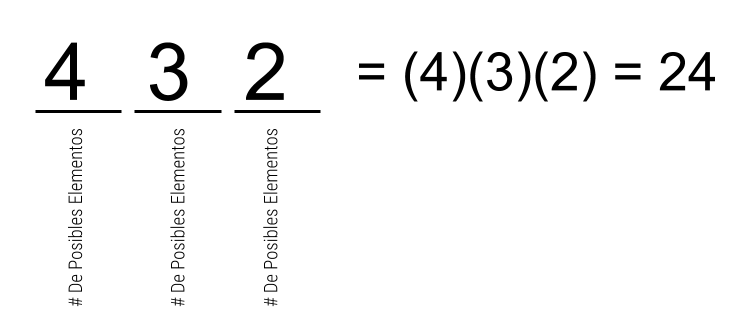
\includegraphics[width=0.6\textwidth]{PermutacionesEjemplo}
                    \end{figure}
                    
                
                \end{SmallIndentation}


        % ==============================================================
        % ===============      COMBINACION        ======================
        % ==============================================================
        \clearpage
        \section{Combinación}

            Una permutación es un arreglo de objetos donde el ordén NO es importante. 

            Entonces definimos a ${}_nC_r$ a la cantidad de muestras sin ordenadas de tamaño r sin remplazo
            de un conjunto de n objetos.

            Entonces decimos que:
            \begin{equation*}
                {n \choose r}
                = {}_nC_r 
                = \dfrac{{}_nP_r}{r!}          
                = \dfrac{n!}{r!(n-r)!}          
                = \dfrac{(n)(n-1)(n-2)\dots(n-r+1)}{r!}
            \end{equation*}

            Esto tiene mucho sentido si lo ves desde otro angulo, pues en cuanto a las permutaciones
            tendremos $(n)(n-1)(n-2)\dots(n-r+1)$, pero resulta que muchas de esas permutaciones son
            basicamente la misma, solo cambiando el orden, así que si el orden ya no importa, es tan sencillo
            como dividir entre la cantidad de veces que podemos ordenar esas permutaciones de tamaño $r$


            % =====================================================
            % ====      COMBINACIONES Y SUBCONJUNTOS       ========
            % =====================================================
            \vspace{1em}
            \subsection{Combinaciones y Subconjuntos}

                Resulta ser que hay dos grande problemas clásicos de teoría de conjuntos
                que podemos resolver con combinaciones:
                \begin{itemize}
                    \item 
                        El número de subconjuntos de cardinalidad $r$ de un conjunto de $n$ elementos
                        \begin{align*}
                            {n \choose r}
                        \end{align*}

                    \item
                        Número de subconjuntos de un conjunto de $n$ elementos:
                        \begin{equation*}
                            \sum_{i = 0}^n {n \choose i} = 2^n
                        \end{equation*}
                \end{itemize}


            % =====================================================
            % =============      EJEMPLOS        ==================
            % =====================================================
            \vspace{1em}
            \subsection{Ejemplos}

                % ======== DEMOSTRACION ========
                \begin{SmallIndentation}[1em]
                    \textbf{Ejemplo 1}:
                    
                    Cuantos equipos se puede formar que incluyan 2 físicos y 1 matemático
                    si se sabe que hay 4 físicos y 3 matemáticos.

                    Ya que no nos importa el orden esto esta mas sencillo de lo que parece:
                    \begin{align*}
                        {4 \choose 2} {3 \choose 1}
                            = \dfrac{4!}{2!(4-2)!}\dfrac{3!}{1!(3-1)!}
                            = 18                     
                    \end{align*}                    
                
                \end{SmallIndentation}
                    


            % ==============================================================
            % ===============        FORMULAS         ======================
            % ==============================================================
            \clearpage
            \subsection{Propiedades Coheficientes Binomiales}

                \begin{itemize}

                    \item 
                        Propiedades Simetrícas
                        \begin{equation*}
                            {n \choose k} = {n \choose n - k}
                        \end{equation*}

                    \item 
                        Casos Especiales
                        \begin{align*}
                            {n \choose 0} = {n \choose n} = 1
                            \MegaSpace \MegaSpace
                            {n \choose 1} = {n \choose n-1} = n   
                        \end{align*}

                    \item 
                        Teorema del Binomio
                        \begin{equation*}
                            (x + y)^n 
                                = \sum_{k=0}^n {n \choose k} x^k y^{n-k}
                        \end{equation*}


                    \item 
                        Teorema del Binomio (Caso Especial)
                        \begin{equation*}
                            \sum_{k=0}^n {n \choose k} p^k (1 - p)^{n-k} = 1
                        \end{equation*}

                \end{itemize}






% //////////////////////////////////////////////////////////////////////////////////////////////////////////
% ///////////////////////       VARIABLES ALEATORIAS DISCRETAS       ///////////////////////////////////////
% //////////////////////////////////////////////////////////////////////////////////////////////////////////
\part{Variables Aleatorias Discretas}
\clearpage



    % ===============================================================================
    % ===============       VARIABLES ALEATORIAS DISCRETAS     ======================
    % ===============================================================================
    \chapter{Variables Aleatorias Discretas}



        % ==============================================================
        % ===========                DEFINICION         ================
        % ==============================================================
        \clearpage
        \section{Variables Aleatorias}

            Una variable aleatoria es una función que asigna a cada elemento $E_i \in S$ en el espacio
            muestral a un número real $X(E_i) \in \Reals$, es decir, en español, lo que hace
            es que es una función que nos da información de una característica de cada elemento
            del espacio muestral.

            Esta se denota con mayúsculas y no es un número, es una función.
            Para poner a un valor posible de una variable aleatoria lo denotamos con minúsculas.

            % ==============================================================
            % =======     VARIABLES ALEATORIAS DISCRETAS       =============
            % ==============================================================
            \vspace{2em}
            \subsection{Variables Aleatorias Discretas}

                Las variables aleatorias cuyo conjunto de valores posibles es finito o infinito contable
                entonces decimos que es una variable aleatoria discreta.

                % ======== EJEMPLO ========
                \begin{SmallIndentation}[1em]
                    \textbf{Ejemplo}:
                    
                    Por ejemplo considera que vas a lanzar 3 monedas, entonces tenemos que:
                    \begin{equation*}
                        S = \Set{ccc, ccx, cxc, xcc, xxc, xcx, cxx, xxx}
                    \end{equation*}

                    Entonces podemos tener una variable aleatoria como:

                    Sea $X =$ Número de caras en 3 lanzamientos.

                    Entonces podemos decir que:
                    \begin{align*}
                        X(ccc) &= 3  \\
                        X(ccx) &= 2  \\
                        X(cxc) &= 2  \\
                        X(xcc) &= 2  \\
                        X(xxc) &= 1  \\
                        X(xcx) &= 1  \\
                        X(cxx) &= 1  \\
                        X(xxx) &= 0
                    \end{align*}

                    Por lo tanto los vales posibles son $0, 1, 2, 3$.

                \end{SmallIndentation}
                


        % ==============================================================
        % ===========      FUNCION PROBABILIDAD         ================
        % ==============================================================
        \clearpage
        \section{Función Probabilidad $f_X$}

            % ======================================================
            % ===========          DEFINICIÓN       ================
            % ======================================================
            \subsection{Definición}

                También se le conoce como función de probabilidad puntual.
                Es una función que toma todos los posibles valores una variable aleatoria y nos regresa un número
                real entre el 0 y el 1 dado por la probabilidad de el valor de la variable aleatoria sea $x$.
                Es decir:
                \begin{equation*}
                    f_X (x) = P(X = x)
                \end{equation*}


            % ======================================================
            % =======         UNIFORME CONTINUA     ================
            % ======================================================
            \subsection{Uniforme Continua}
                \begin{figure}[h]
                    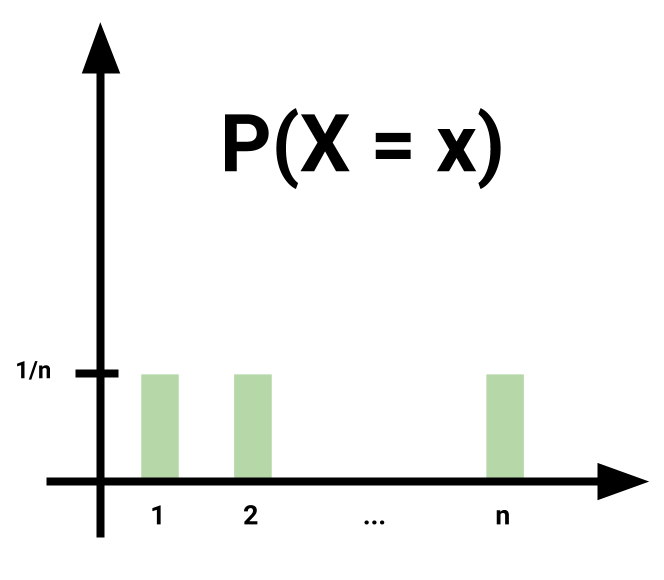
\includegraphics[width=0.45\textwidth]{UniformeDiscreta}
                \end{figure}


            % ======================================================
            % =======              PROPIEDADES      ================
            % ======================================================
            \subsection{Propiedades}

                Es una función de probabilidad, es decir tiene que cumplir que la suma de todos los posibles
                valores de la variable aleatoria den uno.

                Más formalmente tenemos que la función probabilidad es aquella función que cumple que:
                \begin{itemize}
                    \item $\forall a \in \Reals \MegaSpace 0 \leq f_X(a) \leq 1$
                    \item $\Set{x \Such f_X(x) \neq 0}$ es un conjunto finito o numerable
                    \item $\displaystyle \sum_x f_X(x) = 1$
                \end{itemize}

            % ======================================================
            % ===========            EJEMPLOS       ================
            % ======================================================
            \clearpage
            \subsection{Ejemplos}

            % ======== EJEMPLO ========
            \begin{SmallIndentation}[1em]
                \textbf{Ejemplo}:
                
                Por ejemplo podemos definir la probabilidad del ejemplo pasado
                podemos definir la función

                $f_{X}(x) = {3 \choose 3} \Wrap{\frac{1}{2}}^x \Wrap{\frac{1}{2}}^{3-x}$ 
                para $x \in \Set{0, 1, 2, 3}$

                Entonces tenemos que:
                \begin{itemize}
                    \item La probabilidad de que $X = 0$ (caigan 0 caras) es $\frac{1}{8}$ 
                    \item La probabilidad de que $X = 1$ (caigan 1 caras) es $\frac{3}{8}$ 
                    \item La probabilidad de que $X = 2$ (caigan 2 caras) es $\frac{3}{8}$ 
                    \item La probabilidad de que $X = 3$ (caigan 3 caras) es $\frac{1}{8}$ 
                \end{itemize}
            
            \end{SmallIndentation}


        % ==============================================================
        % ===========      FUNCION ACUMULADA            ================
        % ==============================================================
        \clearpage
        \section{Función P. Acumulada $F_X$}

            % ======================================================
            % ===========          DEFINICIÓN       ================
            % ======================================================
            \subsection{Definición}

                Describimos a la función de probabilidad acumulada como:
                \begin{equation*}
                    F_X(x) = \sum_{i \leq x} f_{X}(i)
                \end{equation*}

            % ======================================================
            % ===========          PROPIEADES       ================
            % ======================================================
            \subsection{Propiedades}

                \begin{itemize}
                    \item
                        Una característica muy común es que:
                        \begin{itemize}
                            \item $\lim_{x \to -\infty} F_X (x) = 0$
                            \item $\lim_{x \to \infty} F_X (x) = 1$
                        \end{itemize}
                    \item
                        Si $x_1 \leq x_2$ entonces $F_X(x_1) \leq F_X(x_2)$
                \end{itemize}



            % ======================================================
            % =======     FUNCION FUNDAMENTAL       ================
            % ======================================================
            \subsection{Función Fundametal}

                Podemos ver a la acumulada como una función fundamental, tal que
                podemos escribir a todas las demás:
                \begin{itemize}
                    \item $P(X = x)             = F_X(x) - F_X(x - 1)$
                    \item $P(X < x)             = F_X(x - 1)$
                    \item $P(X \leq x)          = F_X(x)$
                    \item $P(X > x)             = 1 - F_X(x)$
                    \item $P(X \geq x)          = 1 - F_X(x - 1)$
                    \item $P(a \leq X \leq b)   = F_X(b) - F_X(a - 1)$
                    \item $P(a < X \leq b)      = F_X(b) - F_X(a)$
                    \item $P(a \leq X < b)      = F_X(b - 1) - F_X(a)$
                    \item $P(a < X < b)         = F_X(b - 1) - F_X(a - 1)$
                \end{itemize}
                


        % ==============================================================
        % ===========           ESPERANZA O MEDIA       ================
        % ==============================================================
        \clearpage
        \section{Esperanza o Media}

            % ======================================================
            % ===========          DEFINICIÓN       ================
            % ======================================================
            \subsection{Definición}

                Decimos que el valor esperado, esperanza ó media de la variable $X$
                se define como:
                \begin{equation*}
                    \mu_{X} = E(X) = \sum_x \; x \; f_X(x) = \sum_x \; x \; P(X = x)
                \end{equation*}

                Representa un promedio ponderado de los valores posibles de la variable basado en
                sus probabilidades.

                Es decir, si se repitiera el experimiento muchísimas veces el promedio de los resultados
                se iría aproximando a la media.

            % =========================================================
            % ===============        PROPIEDADES      =================
            % =========================================================
            \vspace{1em}
            \subsection{Propiedades}

                \begin{itemize}

                    \item 
                        Si $X$ puede tomar un número infinito de valores entonces la esperanza de 
                        $X$ existe si y solo si $\displaystyle \sum_x |x| f_X(x) < \infty$

                    \item
                        Podemos dar una definición al evaular la esperanza sobre una función:
                        \begin{equation*}
                            E(g(x)) = \sum_x \; g(x) \; f_X(x)    
                        \end{equation*}

                    \item Es un Operador Lineal, es decir:
                        \begin{equation*}
                            E(\alpha X + \beta Y) = \alpha E(X) + \beta E(Y)   
                        \end{equation*}

                    \item
                        Si $X, Y$ son independientes entonces:
                        \begin{equation*}
                            E(XY) = E(X) E(Y)  
                        \end{equation*}

                    \item
                        Si $a$ es una constante, entonces: 
                        \begin{equation*}
                            E(a) = a
                        \end{equation*}

                \end{itemize}


        % ==============================================================
        % ===========              VARIANZA             ================
        % ==============================================================
        \clearpage
        \section{Varianza}

            % ======================================================
            % ===========          DEFINICIÓN       ================
            % ======================================================
            \subsection{Definición}

                Decimos que la varianza de la variable $X$
                con $f_{X}(x)$ se define como:
                \begin{equation*}
                    v(X) = E((X - \mu)^2)
                \end{equation*}

                Podemos decir por su misma definición que la varianza siempre es positiva.

                Es decir, este valor nos indica que tan lejos estan en promedio los valores de
                su misma media, es decir, que tan dispersa o concentrada esta la distribución de 
                los datos.

            % ====================================================
            % ===========    DESVICACIÓN ESTANDAR       ==========
            % ====================================================
            \vspace{1em}
            \subsection{Desvianción Estandar}

                Decimos que la desvianción estandar de la variable $X$
                con $f_{X}(x)$ se define como:
                \begin{equation*}
                    \sigma(X) = \sqrt{v(X)}
                \end{equation*}

                Se usa generalmente por las unidades que tiene la varianza, nada mas


            % ==============================================================
            % ===============        PROPIEDADES      ======================
            % ==============================================================
            \clearpage
            \subsection{Propiedades}

                \begin{itemize}

                    \item
                        $v(X) = E(X^2) - (E(X))^2$

                        % ======== DEMOSTRACION ========
                        \begin{SmallIndentation}[1em]
                            \textbf{Demostración}:
                            
                            Esto esta demasiada sencillo:
                            \begin{align*}
                                v(X) 
                                    &= E((X - \mu)^2)                    \\
                                    &= E(X^2 - 2x\mu +\mu^2)             \\
                                    &= E(X^2) - E(2x\mu) + E(\mu^2)      \\
                                    &= E(X^2) - 2\mu E(x) + E(\mu^2)     \\
                                    &= E(X^2) - 2\mu^2 + \mu^2           \\
                                    &= E(X^2) - \mu^2
                            \end{align*}
                        
                        \end{SmallIndentation}
                            

                    \item 
                        $V(a) = 0$

                        % ======== DEMOSTRACION ========
                        \begin{SmallIndentation}[1em]
                            \textbf{Demostración}:
                            
                            Sea $a = g(X)$, entonces su $\mu = a$, por lo
                            tanto
                            \begin{align*}
                                V(a) 
                                    &= E(a - a)^2)           \\
                                    &= E(0)^2)               \\
                                    &= 0
                            \end{align*}
                        
                        \end{SmallIndentation}

                    \item 
                        $v(aX) = a^2 v(X)$

                        % ======== DEMOSTRACION ========
                        \begin{SmallIndentation}[1em]
                            \textbf{Demostración}:
                            \begin{align*}
                                V(aX) 
                                    &= E(aX^2) - E^2(aX)       \\
                                    &= a^2 E(X^2) - a^2E^2(X)  \\
                                    &= a^2 [E(X^2) - E^2(X)]   \\
                                    &= a^2 [v(X]          
                            \end{align*}
                        
                        \end{SmallIndentation}


                    \item 
                        $v(X + Y) = v(X) + v(Y) + 2Cov(X,Y)$

                        % ======== DEMOSTRACION ========
                        \begin{SmallIndentation}[1em]
                            \textbf{Demostración}:
                            
                            Esta esta larga:
                            \begin{align*}
                                v(X + Y) 
                                    &= E(X + Y)^2 - (E(X+Y))^2                              \\
                                    &= E(X) + E(Y) + 2E(XY) - (E(X+Y))^2                    \\
                                    &= E(X) + E(Y) - (E(X)+E(Y))^2 + 2E(XY)                 \\
                                    &= E(X) + E(Y) - E^2(X)-E^2(Y) + 2E(XY) -2E(X)E(Y)      \\
                                    &= E(X) - E^2(X) + E(Y)-E^2(Y) + 2E(XY) -2E(X)E(Y)      \\
                                    &= v(x) + v(Y) + 2E(XY) - 2E(X)E(Y)                     \\
                                    &= v(x) + v(Y) + 2Cov(X, Y) 
                            \end{align*}
                        
                        \end{SmallIndentation}

                    \clearpage

                    \item 
                        $v(X - Y) = v(X) - v(Y) - 2Cov(X,Y)$

                        % ======== DEMOSTRACION ========
                        \begin{SmallIndentation}[1em]
                            \textbf{Demostración}:
                            
                            Es lo mismo, que la de arriba :v
                        
                        \end{SmallIndentation}
                            

                    \item
                        Si $X$ y $Y$ son independientes, entonces $v(X + Y) = v(X) + v(Y)$

                        % ======== DEMOSTRACION ========
                        \begin{SmallIndentation}[1em]
                            \textbf{Demostración}:
                            
                            Es lo mismo que la de arriba, solo recuerda que si $X, Y$ son independientes
                            entonces tenemos que $Cov(X, Y) = 0$
                        
                        \end{SmallIndentation}
                            

                    \item
                        En general si $X_1, X_2, \dots, X_n$ son variables aleatorias, entonces
                        tenemos que:
                        \begin{align*}
                            v\Wrap{\sum_{i = 1}^n X_i} = \sum_{i = 1}^n v(X_i) + 2\sum_{i < j}^n Cov(X_i, X_j)
                        \end{align*}

                        % ======== DEMOSTRACION ========
                        \begin{SmallIndentation}[1em]
                            \textbf{Demostración}:
                            
                            Es inducción :v
                        
                        \end{SmallIndentation}
                            

                    \end{itemize}
                            


        % ==============================================================
        % ===========            COVARIANZA             ================
        % ==============================================================
        \clearpage
        \section{Covarianza}

            % ======================================================
            % ===========          DEFINICIÓN       ================
            % ======================================================
            \subsection{Definición}

                Sea $X, Y$ dos variables independientes, entonces
                definimos a la covarianza como:
                \begin{equation*}
                    Cov(X, Y)
                        = E\Wrap{(X - \mu_{X})(Y - \mu_{Y})}
                \end{equation*}

                Es una manera de medir la dispersión conjunta de ambas variables.



            
            % =====================================================
            % ===============        PROPIEDADES      =============
            % =====================================================
            \vspace{1em}
            \subsection{Propiedades}

                \begin{itemize}

                    \item 
                        $Cov(X, Y) = E(X Y) - \mu_{X}\mu_{Y}$

                        % ======== DEMOSTRACION ========
                        \begin{SmallIndentation}[1em]
                            \textbf{Demostración}:
                            
                            Podemos demostrar esto, bien facil:
                            \begin{align*}
                                Cov(X, Y)
                                    &= E\Wrap{(X - \mu_X)(Y - \mu_Y)}                   \\
                                    &= E\Wrap{XY - X\mu_Y -\mu_XY - \mu_X\mu_Y}         \\
                                    &= E(XY) - E(X\mu_Y) -E(\mu_XY) + E(\mu_X\mu_Y)     \\
                                    &= E(XY) - \mu_YE(X) -\mu_XE(Y) +  E(\mu_X\mu_Y)    \\
                                    &= E(XY) - \mu_Y\mu_X -\mu_X\mu_Y + E(\mu_X\mu_Y)   \\
                                    &= E(XY) - \mu_Y\mu_X -\mu_X\mu_Y + \mu_X\mu_Y      \\
                                    &= E(XY) - \mu_Y\mu_X
                            \end{align*}
                        
                        \end{SmallIndentation}

                    \item La covarianza de 2 variables independientes es cero

                    % ======== DEMOSTRACION ========
                    \begin{SmallIndentation}[1em]
                        \textbf{Demostración}:
                        
                        Mira esto:
                        \begin{align*}
                            Cov(X, Y)
                                &= E(XY) - \mu_Y\mu_X                           
                                    && \Remember{Si es que son independientes}      \\
                                &= E(X)E(Y) - \mu_Y\mu_X
                                    && \Remember{Recuerda que $E(X) = \mu_X$}       \\
                                &= 0
                        \end{align*}
                    
                    \end{SmallIndentation}
                        
                            
                \end{itemize}




        % ==============================================================
        % ===========        MOMENTOS CENTRALES         ================
        % ==============================================================
        \clearpage
        \section{Momentos Centrales}

            Si $X$ es una variable aleatoria tal que $E(X) = \mu_x$ entonces tenemos que:
            \begin{itemize}
                \item 
                    El k-ésimo momento central esta definida como:
                    \begin{equation}
                        \mu_k^c 
                            = E\Brackets{(X - \mu)^k}
                            = \sum_x (x - \mu)^k P(X = x)
                    \end{equation}

                \item 
                    El k-ésimo momento alrededor del origen esta definida como:
                    \begin{equation}
                        \mu_k^0 
                            = E\Wrap{X^k}
                            = \sum_x x^k P(X = x)
                    \end{equation}

            \end{itemize}



            % ==============================================================
            % ===============        PROPIEDADES      ======================
            % ==============================================================
            \subsection{Propiedades}

                \begin{itemize}

                    \item
                        Ya hemos trabajo con momentos, veamos algunos:

                        \begin{itemize}
                            \item 
                                \textbf{La Esperanza}

                                Esta se puede ver como el primer momento alrededor del origen

                                $\mu_X = \mu_1^0$

                            \item 
                                \textbf{La Varianza}

                                Esta se puede ver como el primer momento alrededor central
                                \begin{equation*}
                                    v(X) = E[(X - \mu)^2] = \mu_2^c    
                                \end{equation*}

                                O bien podemos verlo como $v(X) = E(X^2) - \mu^2$ donde $E(X^2)$
                                es un segundo momento alrededor del origen

                         \end{itemize}

                \end{itemize}


            % ==============================================================
            % ===========     FUNCION GENERADORA      ======================
            % ==============================================================
            \clearpage
            \subsection{Función Generadora de Momentos}

                La podemos definir como:
                \begin{equation*}
                    \Psi_X (t) 
                        = E(e^{tX})
                        = \sum_x \; e^{tx} \; P(X = x)
                \end{equation*}

                Solemos decir que la k-ésima derivada de la función generadora
                de momentos evaluada en $t = 0$ da como resultado el k-ésimo momento central al origen

                Es decir, siguen el siguiente patrón:
                \begin{itemize}
                    \item $\Psi_X' (t = 0) = E(X)$ 
                    \item $\Psi_X'' (t = 0) = E(X^2)$ 
                    \item $\Psi_X''' (t = 0) = E(X^3)$ 
                    \item $\Psi_X^{(n)} (t = 0) = E(X^n)$ 
                \end{itemize}



            % ==============================================================
            % ===============        PROPIEDADES      ======================
            % ==============================================================
            \clearpage
            \subsection{Propiedades}

                \begin{itemize}

                    \item
                        Nota que $\Psi_x(a) = E(e^{aX})$

                    \item
                        Si $Y = aX + b$ entonces tenemos que:

                        $\Psi_Y(t) = e^{bt} \Psi_X(at)$

                        % ======== DEMOSTRACION ========
                        \begin{SmallIndentation}[1em]
                            \textbf{Demostración}:
                            
                            Esta esta fácil, sea $Y = aX + b$:
                            \begin{align*}
                                \Psi_Y(t) 
                                    &= E(e^{tY})                    \\
                                    &= E(e^{t(aX + b)})             \\
                                    &= E(e^{at X + tb})             \\
                                    &= E(e^{at X} e^{tb})           \\
                                    &= e^{tb} E(e^{at X})           \\
                                    &= e^{tb} \Psi_X(at)
                            \end{align*}
                        
                        \end{SmallIndentation}
                            

                    \item
                        $\Psi_X (t = 0) = \mu_k$

                    \item
                        $\Psi_X (t = 0) = E(X)$

                    \item
                        Nota que si tuvieramos un montón de variables aleatorias
                        $X_1, X_2, X_3, \dots, X_n$
                        Y decimos que $\displaystyle Y = \sum_{i = 1}^n X_i$

                        Entonces tenemos que:
                        \begin{equation*}
                            \Psi_Y(t) = \prod_{i = 1}^n \Psi_{X_i}(t)
                        \end{equation*}

                        % ======== DEMOSTRACION ========
                        \begin{SmallIndentation}[1em]
                            \textbf{Demostración}:
                            
                            Esta también es importante:
                            \begin{align*}
                                \Psi_Y(t)
                                    &= E\Wrap{e^{tY}}                       \\
                                    &= E\Wrap{e^{t\sum_{i = 1}^n X_i}}      \\
                                    &= E\Wrap{\prod_{i = 1}^n e^{X_i}}      \\
                                    &= \prod_{i = 1}^n E\Wrap{e^{X_i}}      \\
                                    &= \prod_{i = 1}^n \Psi_{X_i}(t)
                            \end{align*}
                        
                        \end{SmallIndentation}


                \end{itemize}






    % ===============================================================================
    % ===============       DISTRIBUCIONES DISCRETAS FAMOSAS     ====================
    % ===============================================================================
    \chapter{Distribuciones Famosas}


        % ==============================================================
        % ====                  BERNOULLI                   ============
        % ==============================================================
        \clearpage
        \section{Bernoulli}


            % ==============================================================
            % ==============          DEFINICION           =================
            % ==============================================================
            \subsection{Definición}

                Suponte un experimento en el que solo tienes dos salidas, 
                $0, 1$, $0$ para el fracaso y $1$ para el exito,
                suponte que la probabilidad de que salga $1$ es $p$
                y la que salga $0$ es $q = 1 - p$.


                % ======================================================
                % =========    VARIABLE ALEATORIA       ================
                % ======================================================
                \vspace{1em}
                \subsubsection{Variable Aleatoria}

                    Ahora, nuestra variable aleatoria sera:
                    \begin{equation*}
                        X : \text{Resultado del experimento}
                    \end{equation*}

                    Ahora, los valores posibles que puede tomar son muy muy sencillos, basicamente porque
                    solo hay 2 opciones, o salio bien, o salio mal, es decir $X$ puede tomar los valores
                    $0, 1$.

                    Solemos entonces escribir esta distribución como:
                    \begin{equation*}
                        X \sim Ber(x; p)
                    \end{equation*}

                    donde:
                    \begin{itemize}
                        \item $x$: Nuestra variable
                        \item $p$: Probabilidad de Exito
                    \end{itemize}


            % ==============================================================
            % ==========     FUNCIÓN PROBABILIDAD          =================
            % ==============================================================
            \clearpage
            \subsection{Función Probabilidad}

                Esta es clásica:
                \begin{align*}
                    f_X(x) = (p^x) ((1-p)^{1-x}) = p^x q^{1-x}
                \end{align*}

                % ======== DEMOSTRACION ========
                \begin{SmallIndentation}[1em]
                    \textbf{Demostración}:
                    
                    Esta esta fácil, podemos hacerla por partes, como parece
                    más natural y ver que:
                    \begin{align*}
                        F_X(x) = 
                            \begin{cases}
                                q \Space& x = 0             \\
                                p \Space& x = 1             \\
                            \end{cases}
                    \end{align*}

                    Podemos extender esta idea de muchas maneras a una expresión
                    la que damos es solo una de ellas.
                
                \end{SmallIndentation}
                    
            % ==============================================================
            % =========   FUNCION PROBABILIDAD ACUMULADA        ============
            % ==============================================================
            \vspace{1em}
            \subsection{Función P. Acumulada}

                Por definición tenemos que:
                \begin{align*}
                    F_X(x) = 
                        \begin{cases}
                            0 \Space& x < 0             \\
                            q \Space& 0 \leq x < 1      \\
                            p \Space& 1 \leq x 
                        \end{cases}
                \end{align*}

                Y esta conviene mejor dejarla así.

            % ==============================================================
            % =========          FUNCION ESPERANZA              ============
            % ==============================================================
            \clearpage
            \subsection{Esperanza}

                Esta es la distribución con la esperanza más fácil que veras:
                \begin{align*}
                    E(X) = p
                \end{align*}

                % ======== DEMOSTRACION ========
                \begin{SmallIndentation}[1em]
                    \textbf{Demostración}:
                    
                    Nota que por definición tenemos que:
                    \begin{align*}
                        \mu_X 
                            &= \sum_x x P(X = x)        \\
                            &= 0(q) + 1(p)              \\
                            &= p
                    \end{align*}
                    
                
                \end{SmallIndentation}


            % ==============================================================
            % =========          FUNCION VARIANZA               ============
            % ==============================================================
            \vspace{1em}
            \subsection{Varianza}

                Esta es igualmente sencilla:
                \begin{align*}
                    v(X) = p(1-p) = p - p^2 = pq
                \end{align*}

                % ======== DEMOSTRACION ========
                \begin{SmallIndentation}[1em]
                    \textbf{Demostración}:
                    
                    Por definición tenemos que:
                    \begin{align*}
                        v(X)
                            &= E(x^2) - \mu^2               \\
                            &= E(x^2) - p^2                 \\
                            &= \sum_x x^2 P(X = x) - p^2    \\
                            &= 0(q) + 1(p) - p^2            \\
                            &= p - p^2                      \\
                            &= p(1 - p)                     \\
                            &= pq
                    \end{align*}
                
                \end{SmallIndentation}
                        

            % ==============================================================
            % =========   FUNCION GENERADORA DE MOMENTOS        ============
            % ==============================================================
            \clearpage
            \subsection{Función Generadora}

                Esta igual es muy bonita:
                \begin{align*}
                    \Psi(t) = (q) + e^t(p)
                \end{align*}

                % ======== DEMOSTRACION ========
                \begin{SmallIndentation}[1em]
                    \textbf{Demostración}:
                    
                    Por definición tenemos que:
                    \begin{align*}
                        \Psi(t) 
                            &= E(e^tX)                      \\
                            &= \sum_x e^tx P(X = x)         \\
                            &= e^{0t}(q) + e^{1t}(p)        \\
                            &= (q) + e^t(p)   
                    \end{align*}
                
                \end{SmallIndentation}
                    

        % ==============================================================
        % ====                  BINOMIAL                    ============
        % ==============================================================
        \clearpage
        \section{Binomial}

            % ==============================================================
            % ==============          DEFINICION           =================
            % ==============================================================
            \subsection{Definición}

                Un experimento binomial consiste en $n$ ensayos Bernoulli
                independientes, con una probabilidad de exito individual constante.

                La variable aleatoria discreta es el número de exitos de los experimentos individuales
                donde sus posibles valores fueron $X = \Set{0, 1, \dots, n}$.

                Observa que la variable aleatoria se puede ver como la suma de Bernoullis independientes,
                es decir $X = X_1 + X_2 + X_3 + \dots + X_n$

                % ======================================================
                % =========    VARIABLE ALEATORIA       ================
                % ======================================================
                \vspace{1em}
                \subsubsection{Variable Aleatoria}

                    Ahora, nuestra variable aleatoria sera:
                    \begin{equation*}
                        X : \text{Número de Exitos en los experimentos}
                    \end{equation*}

                    Ahora, los valores posibles que puede tomar son muy muy sencillos, suponte que haremos
                    n experimentos, entonces $X$ tiene que tomar valores entre $0 \dots n$

                    Solemos entonces escribir esta distribución como:
                    \begin{equation*}
                        X \sim Bin(x; n, p)
                    \end{equation*}

                    donde:
                    \begin{itemize}
                        \item $x$: Nuestra variable
                        \item $p$: Probabilidad de Exito de cada experimiento Bernoulli
                    \end{itemize}


            % ==============================================================
            % ==========     FUNCIÓN PROBABILIDAD          =================
            % ==============================================================
            \clearpage
            \subsection{Función Probabilidad}
            
                Esta esta fácil:
                \begin{align*}
                    f_X(x) 
                        = {n \choose x} p^x q^{n - x}
                \end{align*}

                % ======== DEMOSTRACION ========
                \begin{SmallIndentation}[1em]
                    \textbf{Demostración}:
                    
                    ¿Porque? Porque estamos hablando de eventos independientes por lo
                    tanto su probabilidad conjunta es el producto de las individuales, 
                    y literlalmente estamos usando la definición de combinación.
                
                \end{SmallIndentation}
                        

            % ==============================================================
            % =========   FUNCION PROBABILIDAD ACUMULADA        ============
            % ==============================================================
            \vspace{1em}
            \subsection{Función P. Acumulada}

                    Esta esta fácil:
                    \begin{align*}
                        F_X(x) = \sum_{i=0}^x {n \choose i}p^i q^{n - i}
                    \end{align*}

                    % ======== DEMOSTRACION ========
                    \begin{SmallIndentation}[1em]
                        \textbf{Demostración}:
                        
                        Literalmente es la definición.
                    
                    \end{SmallIndentation}
                   
            % ==============================================================
            % =========   FUNCION GENERADORA DE MOMENTOS        ============
            % ==============================================================
            \clearpage
            \subsection{Función Generadora}  

                Por definición tenemos que:
                \begin{align*}
                    \Psi (t) = \Wrap{q + e^tp}^n   
                \end{align*}

                % ======== DEMOSTRACION ========
                \begin{SmallIndentation}[1em]
                    \textbf{Demostración}:
                    
                    Espera, espera, me explico mejor, lo que pasa es la binomial se puede ver
                    como una suma de variables independientes entonces solo basta con recordar
                    que ya demostramos que la función generadora de momentos de una suma
                    de variables independientes es el producto de la función generadora
                    de momentos de cada una.

                    Es decir:
                    \begin{align*}
                        \Psi_X (t) 
                            &= \prod_{i = 1}^n \Psi_{X_i} (t)   \\
                            &= \prod_{i = 1}^n \Psi_{X_i} (t)   \\
                            &= \prod_{i = 1}^n q + e^t p        \\
                            &= \Wrap{q + e^tp}^n                  
                    \end{align*} 

                \end{SmallIndentation}
                    
            % ==============================================================
            % =========          FUNCION ESPERANZA              ============
            % ==============================================================
            \vspace{1em}
            \subsection{Esperanza}  

                Esta también es sencilla:
                \begin{align*}
                    E(X) = np
                \end{align*}

                % ======== DEMOSTRACION ========
                \begin{SmallIndentation}[1em]
                    \textbf{Demostración}:
                    
                    Podemos usar que la variable aleatoria se puede ver como la suma
                    de Bernoullis independientes.

                    Es decir $X = \sum_x X_i$

                    \begin{align*}
                        \mu_X 
                            &= E(X)                 \\
                            &= E(\sum_x X_i)        \\
                            &= \sum_x E(X_i)        \\
                            &= np
                    \end{align*}
                    
                \end{SmallIndentation}


            % ==============================================================
            % =========          FUNCION VARIANZA               ============
            % ==============================================================
            \vspace{1em}
            \subsection{Varianza}

                Esta es bonita también:
                \begin{align*}
                    v(X) = npq   
                \end{align*}

                % ======== DEMOSTRACION ========
                \begin{SmallIndentation}[1em]
                    \textbf{Demostración}:
                    
                    Esta la haremos usando propiedades de la varianza, recuerda que
                    son la suma de eventos independientes:
                    \begin{align*}
                        v(X) 
                            &= v\Wrap{\sum_{i=0}^n X_i}         \\
                            &= \sum_{i=1}^n v(X_i)              \\
                            &= \sum_{i=1}^n pq                  \\
                            &= npq
                    \end{align*}
                
                \end{SmallIndentation}
                    
                    
            % ==============================================================
            % =========          PROPIEDADES                    ============
            % ==============================================================
            \clearpage
            \subsection{Propiedades}

                \begin{itemize}
                    
                    \item 
                        Sean $X_1, X_2, \dots, X_k$ $k$ variables aleatorias discretas independientes
                        y $X_i \sim Bin(x_i; n_i, p)$ con $i = 1, 2, \dots, k$.

                        Entonces la variable aleatoria $X = X_1 + X_2 + \dots + X_k$ tiene una 
                        distribución binomial tal que $X \sim Bin\Wrap{x; \sum_{i=1}^k n_i, p}$ 

                        % ======== DEMOSTRACION ========
                        \begin{SmallIndentation}[1em]
                            \textbf{Demostración}:
                            
                            Veamos que:
                            \begin{align*}
                                \Psi_X(t)
                                    &= \Psi_{X_1 + X_2 + \dots + X_k}(t)                        \\
                                    &= \prod_{i=1}^k \Psi_{X_i}                                 \\
                                    &= (q +pe^t)^{n_1}(q +pe^t)^{n_2} \dots (q +pe^t)^{n_k}     \\
                                    &= (q +pe^t)^{\sum_{i=i}^k n_i}
                            \end{align*}

                            Es decir $\Psi_X(t) = (q +pe^t)^n$ con $n = \sum_{i=i}^k n_i$, es decir
                            vimos que $X \sim Bin\Wrap{x; \sum_{i=1}^k n_i, p}$
                            
                        
                        \end{SmallIndentation}


                \end{itemize}

                    
                    


        % ==============================================================
        % ====                  GEOMETRICA                  ============
        % ==============================================================
        \clearpage
        \section{Geométrica}

            % ==============================================================
            % ==============          DEFINICION           =================
            % ==============================================================
            \subsection{Definición}

                Supón que se repiten de manera independiente ensayos Bernoulli
                con una probabilidad de exito constante de $p$ hasta obtener el primer
                exito.

                La variable discreta es el número de experimentos hasta un primer exito
                donde sus posibles valores fueron $X = \Set{1, 2, 3, \dots}$.


                % ======================================================
                % =========    VARIABLE ALEATORIA       ================
                % ======================================================
                \vspace{1em}
                \subsubsection{Variable Aleatoria}

                    Ahora, nuestra variable aleatoria sera:
                    \begin{equation*}
                        X : \text{Número de experimentos hasta un exito}
                    \end{equation*}

                    Ahora, los valores posibles que puede tomar son muy muy sencillos,
                    porque puede que pase en el primer experimento o en el segundo, 
                    es decir la variable aleatoria puede tomar cualquier valor en los enteros
                    positivos.

                    Solemos entonces escribir esta distribución como:
                    \begin{equation*}
                        X \sim G(x; p)
                    \end{equation*}

                    donde:
                    \begin{itemize}
                        \item $x$: Nuestra variable
                        \item $p$: Probabilidad de Exito de cada experimento Bernoulli
                    \end{itemize}


            % ==============================================================
            % ==========     FUNCIÓN PROBABILIDAD          =================
            % ==============================================================
            \clearpage
            \subsection{Función Probabilidad}

                Esta esta fácil:
                \begin{align*}
                    f_X(x) = q^{x - 1} \; p
                \end{align*}

                Es decir, es la propabilidad de que todos los anteriores sean
                fracasos y el actual sea el exito.


            % ==============================================================
            % =========   FUNCION PROBABILIDAD ACUMULADA        ============
            % ==============================================================
            \vspace{1em}
            \subsection{Función P. Acumulada}

                Esta también es sencilla:
                \begin{align*}
                    F_X(x) = 1 - q^x
                \end{align*}

                % ======== DEMOSTRACION ========
                \begin{SmallIndentation}[1em]
                    \textbf{Demostración}:
                    
                    Esta esta fácil, solo espero que recuerdes
                    la suma de la serie geométrica:
                    \begin{align*}
                        F_X(x) 
                            &= \sum_{i=1}^x pq^{i - 1}      \\
                            &= (p)\sum_{i=0}^{x-1} q^i      \\
                            &= (p)\frac{1-q^x}{1-q}         \\
                            &= (p)\frac{1-q^x}{p}           \\
                            &= 1-q^x
                    \end{align*}
                
                \end{SmallIndentation}
                    

            % ==============================================================
            % =========          FUNCION ESPERANZA              ============
            % ==============================================================
            \clearpage
            \subsection{Esperanza}

                Esta es muy famosa, y lo repito, que no se te olvide la geométrica
                \begin{align*}
                    E(X) = \frac{1}{p}
                \end{align*}

                % ======== DEMOSTRACION ========
                \begin{SmallIndentation}[1em]
                    \textbf{Demostración}:
                    \begin{align*}
                         E(X)
                            &= \sum_{x=1}^\infty xP(X = x)                          \\
                            &= \sum_{x=1}^\infty x q^{x - 1}p                       \\
                            &= p\sum_{x=1}^\infty x q^{x - 1}                       \\
                            &= p \MiniDerivate \sum_{x=1}^\infty x q^{x - 1}        \\
                            &= p \MiniDerivate \sum_{x=1}^\infty q^x                \\
                            &= p \MiniDerivate \frac{1}{1 - q}                      \\
                            &= p \frac{1}{(1- q)^2}                                 \\
                            &= p \frac{1}{p^2}                                      \\
                            &= \frac{1}{p}                                  
                    \end{align*}    
                
                \end{SmallIndentation}
                      
            % ==============================================================
            % =========          FUNCION VARIANZA               ============
            % ==============================================================
            \clearpage
            \subsection{Varianza}

                Esta también es sencilla:
                \begin{align*}
                    v(X) = \frac{1-p}{p^2}
                \end{align*}

                % ======== DEMOSTRACION ========
                \begin{SmallIndentation}[1em]
                    \textbf{Demostración}:
                    
                    \begin{align*}
                        v(X) 
                            &= E(X^2) - \mu^2                                           \\
                            &= E(X^2) - \frac{1}{p^2}                                   \\
                            &= \sum_{x=1}^\infty x^2P(X = x) - \frac{1}{p^2}            \\
                            &= \sum_{x=1}^\infty x^2 p q^{x-1} - \frac{1}{p^2}          \\
                            &= p\sum_{x=1}^\infty x^2 q^{x-1} - \frac{1}{p^2}           \\
                            &= p\frac{1+q}{(1-q)^3} - \frac{1}{p^2}                     \\
                            &= \frac{1+q}{p^2} - \frac{1}{p^2}                          \\
                            &= \frac{q}{p^2}                                            \\
                            &= \frac{1-p}{p^2}
                    \end{align*}
                
                \end{SmallIndentation}

                 
            % ==============================================================
            % =========   FUNCION GENERADORA DE MOMENTOS        ============
            % ==============================================================
            \clearpage
            \subsection{Función Generadora}   

                Esta también saldra por definición no somos cobardes:
                \begin{align*}
                    \Psi (t) = \frac{pe^t}{1-qe^t}  
                \end{align*}

                % ======== DEMOSTRACION ========
                \begin{SmallIndentation}[1em]
                    \textbf{Demostración}:
                    
                    Por definición tenemos que:
                    \begin{align*}
                        \Psi (t) = E\Wrap{e^{tX}}                                       \\
                        \Psi (t) = \sum_{x=1}^\infty e^{tx} q^{x-1}p                    \\
                        \Psi (t) = p \sum_{x=1}^\infty e^{tx} q^{x-1}                   \\
                        \Psi (t) = p \sum_{x=1}^\infty e^{tx} q^{x-1}                   \\
                        \Psi (t) = p e^t \sum_{x=1}^\infty (qe^t)^x                     \\
                        \Psi (t) = p e^t \frac{1}{1 - qe^t}                             \\
                        \Psi (t) = \frac{pe^t}{1-qe^t} 
                    \end{align*}
                
                \end{SmallIndentation}
                    

            % ==============================================================
            % ====                  PROPIEDADES                 ============
            % ==============================================================
            \clearpage
            \subsubsection{Propiedades}

                \begin{itemize}
                    \item Sea $P(X > a) = q^a$ con $a$ un natural positivo

                        % ======== DEMOSTRACION ========
                        \begin{SmallIndentation}[1em]
                            \textbf{Demostración}:
                            \begin{align*}
                                P(Y > a)
                                    &= 1 - F_X(a)      
                                        && \Remember{Definición de Acumulada}   \\
                                    &= 1 - (1 - q^a)    
                                        && \Remember{Talacha}                   \\
                                    &= q^a    
                                        && \Remember{Bingo}
                            \end{align*}    
                        
                        
                        \end{SmallIndentation}

                    \item Sea $P(X > a + b \Such X > a) = P(X > b)$ con $a, b$ un naturales positivos

                        % ======== DEMOSTRACION ========
                        \begin{SmallIndentation}[1em]
                            \textbf{Demostración}:
                            \begin{align*}
                                P(X > a + b \Such X > a)
                                    &= \frac{P(X > a + b \text{ y } X > a)}{P(X > a)}    
                                        && \Remember{Definición de Condicional}     \\
                                    &= \frac{P(X > a + b)}{P(X > a)}    
                                        && \Remember{Sentido común}                 \\
                                    &= \frac{p^{a+b}}{p^a}
                                        && \Remember{Teorema pasado}                \\
                                    &= p^{(a+b)-a}
                                        && \Remember{Exponentes}                    \\
                                    &= p^b
                                        && \Remember{Usando teorema pasado}         \\
                                    &= P(X > b)
                            \end{align*}    
                        
                        
                        \end{SmallIndentation}
                            
                \end{itemize}


                

        % ==============================================================
        % ==========     HIPER -GEOMETRICA                  ============
        % ==============================================================
        \clearpage
        \section{Hiper-Geométrica}

            % ==============================================================
            % ==============          DEFINICION           =================
            % ==============================================================
            \subsection{Definición}

                Supongamos que tenemos una población de tamaño $r$, ahora
                esta particionado de 2 maneras, como elementos del tipo $r_1$
                o $r_2$.

                Ahora vamos a tomar una muestra aleatoria de tamaño $n$ sin reemplazo
                ni sustitución.

                Ahora, solo por notación si es que $n$, es decir la muestra es menor
                que nuestra población $r$ la llamamos muestra, pero si $n = r$ entonces
                decimos que es un censo.

                % ======================================================
                % =========    VARIABLE ALEATORIA       ================
                % ======================================================
                \space{1em}
                \subsubsection{Variable Aleatoria}

                    Ahora, nuestra variable aleatoria sera:
                    \begin{equation*}
                        X : \text{Número de elementos del tipo $r_1$ en una muestra aleatoria de tamaño $n$}
                    \end{equation*}

                    Ahora, los valores posibles que puede tomar es $max(0, n - r_2) \leq x \leq min(r_1, n)$
                    Ahora, ¿Porque esos números tan feos?
                    Por un lado tenemos que que lo peor que nos puede pasar son dos cosas, o bien su tu
                    muestra es muy pequeña $n$ compara con todo el espacio $r$ y $r_1$ entonces
                    entonces bien que puedes tener toda la mala suerte de que todas caigan donde tu no querías
                    por lo tanto, podría pasar que $X = 0$, pero, pero que pasaría que tu $n$ fuera
                    lo suficientemente grande tal que si que si entrará todo tus fragmentos que no quieres
                    entonces lo mínimo que puede entrar es $n - r_2$.

                    El cálculo para el límite mayor es parecido.


                    Solemos entonces escribir esta distribución como:
                    \begin{equation*}
                        X \sim H(x; n, r_1, r_2)
                    \end{equation*}

                    donde:
                    \begin{itemize}
                        \item $x$: Nuestra variable
                        \item $n$: Tamaño de la muestra
                        \item $r$: Tamaño de TODA la población
                        \item $r_1$: Tamaño de nuestra población de interes
                        \item $r_2$: Tamaño de la población que no es de interes, sale de $r_2 = r - r_1$
                    \end{itemize}


            % ==============================================================
            % ==========     FUNCIÓN PROBABILIDAD          =================
            % ==============================================================
            \clearpage
            \subsection{Función Probabilidad}

                Esta esta muy interesante, es:
                \begin{equation*}
                    f_X(x) = \dfrac{{r_1 \choose x}{r_2 \choose n-x} }{{r \choose n}}
                \end{equation*}

                % ======== DEMOSTRACION ========
                \begin{SmallIndentation}[1em]
                    \textbf{Idea de la Demostración}:
                    
                    Antes que nada, mira lo bonito que sale, arriba tienes $r_1, r_2$ y $r_1+r_2=r$
                    y abajo tienes que $n-x, x$ y $n-x+x = n$
                    
                    Ahora, abajo estamos colocando las posibles formas de escojer conjunto de $n$
                    elementos de una espacio de $r$ elementos, y arriba es la probabilidad
                    conjunta de que primero tengamos $x$ elementos de $r_1$ y $n-x$ elementos de $r_2$
                
                \end{SmallIndentation}
                    

            % ==============================================================
            % =========   FUNCION PROBABILIDAD ACUMULADA        ============
            % ==============================================================
            \vspace{1em}
            \subsection{Función P. Acumulada}

                Esta esta muy interesante, es:
                \begin{align*}
                    F_X(x) 
                        = P(X \leq x)              
                        = \dfrac{1}{\binom{r}{n}}                      
                            \sum_{i = max (0, n - r_2)}^x                
                                \binom{r_1}{i} \binom{r_2}{n - i}
                \end{align*}

                % ======== DEMOSTRACION ========
                \begin{SmallIndentation}[1em]
                    \textbf{Idea de la Demostración}:
                    
                    Es por definición men :v
                
                \end{SmallIndentation}
                    


            % ==============================================================
            % =========          FUNCION ESPERANZA              ============
            % ==============================================================
            \clearpage
            \subsection{Esperanza}

                Esta esta muy interesante:
                \begin{align*}
                    E(X) = n \pfrac{r_1}{r}                    
                \end{align*}

                % ======== DEMOSTRACION ========
                \begin{SmallIndentation}[1em]
                    \textbf{Demostración}:
                    
                    Primero que nada porque usando la definición o algo así nos van a
                    salir cosas horribles, así que mejor empecemos por otro lado.

                    Sea $X_i$ variables aleatorias de Bernoulli, tal que esten
                    definidas por: 
                    \begin{align*}
                        X_i = 
                            \begin{cases}
                                1 & \text{Si $X_i$ es de tipo $r_1$}        \\
                                0 & \text{Si $X_i$ no es de tipo $r_1$}
                            \end{cases}
                    \end{align*}

                    Ahora, como son variables de Bernoulli, podemos encontrar bien facil
                    su esperanza como $E(X_i) = p = \dfrac{r_1}{r}$

                    Ahora, como ya te esperabas, nota que nuestra variable aleatoria hipergeometrica
                    es la suma de las otras $X = \sum_{i = 1}^n X_i$

                    Ahora como la esperanza es un bonito operador lineal tenemos que:
                    \begin{align*}
                        E(X)
                            &= E \Wrap{\sum_{i = 1}^n X_i}      \\
                            &= \sum_{i = 1}^n E(X_i)            \\
                            &= \sum_{i = 1}^n \frac{r_1}{r}     \\
                            &= n \pfrac{r_1}{r}   
                    \end{align*}
                    
                
                \end{SmallIndentation}
                    

                


            % ==============================================================
            % =========   FUNCION GENERADORA DE MOMENTOS        ============
            % ==============================================================
            \clearpage
            \subsection{Función Generadora}

                Esta esta muy interesante, es:
                \begin{align*}
                    \Psi_X(t) 
                        = E( e^{tX} )                 
                        = \dfrac{1}{\binom{r}{n}}                      
                            \sum_{i = max (0, n - r_2)}^{min(n, r_1)}               
                               e^{ti} \binom{r_1}{i} \binom{r_2}{n - i}
                \end{align*}





        % ==============================================================
        % ==========             POISSON                    ============
        % ==============================================================
        \clearpage
        \section{Poisson}


            % ======================================================
            % =========    VARIABLE ALEATORIA       ================
            % ======================================================
            \vspace{1em}
            \subsubsection{Variable Aleatoria}

                La variable aleatoria que cuenta el número de ocurrencías en un periodo
                de tiempo o espacio físico dado se le llama Poisson.

                \begin{equation*}
                    X : \text{Número de ocurrencias en un periodo de tiempo o espacio dado}
                \end{equation*}

                Ahora, los valores posibles que puede tomar es $0, 1, 2, \dots$

                Solemos entonces escribir esta distribución como:
                \begin{equation*}
                    X \sim P(x; \lambda)
                \end{equation*}

                donde:
                \begin{itemize}
                    \item $x$: Nuestra variable
                    \item $\lambda$: Es el número promedio de ocurrencias en el periodo o espacio dado
                \end{itemize}


            % ==============================================================
            % ==========     FUNCIÓN PROBABILIDAD          =================
            % ==============================================================
            \clearpage
            \subsection{Función Probabilidad}

                Esta esta muy interesante, es:
                \begin{equation*}
                    f_X(x) = P(X = x) = e^{- \lambda} \dfrac{\lambda^x}{x!}
                \end{equation*}


            % ==============================================================
            % =========   FUNCION PROBABILIDAD ACUMULADA        ============
            % ==============================================================
            \vspace{1em}
            \subsection{Función P. Acumulada}

                Esta esta muy interesante, es:
                \begin{align*}
                    F_X(x) 
                        = P(X \leq x)              
                        = e{-\lambda}\sum_{i = 0}^x \dfrac{\lambda^i}{i!}
                \end{align*}

                % ======== DEMOSTRACION ========
                \begin{SmallIndentation}[1em]
                    \textbf{Idea de la Demostración}:
                    
                    Es por definición men :v
                
                \end{SmallIndentation}
                    

            % ==============================================================
            % =========   FUNCION GENERADORA DE MOMENTOS        ============
            % ==============================================================
            \clearpage
            \subsection{Función Generadora}

                Esta esta muy interesante, es:
                \begin{align*}
                    \Psi_X(t) 
                        = e^{\lambda(e^t - 1)}
                \end{align*}

                % ======== DEMOSTRACION ========
                \begin{SmallIndentation}[1em]
                    \textbf{Demostración}:
                    
                    Usando la función probabilidad puntual tenemos que:
                    \begin{align*}
                        \Psi_X(t) 
                            &= E( e^{tX} )                                                       \\
                            &= \sum_{x = 0}^\infty e^{tx} P(X = x)                               \\
                            &= \sum_{x = 0}^\infty e^{tx} e^{- \lambda} \dfrac{\lambda^x}{x!}    \\
                            &= e^{- \lambda} \sum_{x = 0}^\infty e^{tx} \dfrac{\lambda^x}{x!}    \\
                            &= e^{- \lambda} \sum_{x = 0}^\infty \dfrac{(e^t \lambda)^x}{x!}     \\
                            &= e^{- \lambda} e^{e^t \lambda}                                     \\   
                            &= e^{\lambda(e^t - 1)}
                    \end{align*}
                
                \end{SmallIndentation}
                    

            % ==============================================================
            % =========          FUNCION ESPERANZA              ============
            % ==============================================================
            \clearpage
            \subsection{Esperanza}

                Esta esta muy interesante:
                \begin{align*}
                    E(X) = \lambda               
                \end{align*}

                % ======== DEMOSTRACION ========
                \begin{SmallIndentation}[1em]
                    \textbf{Demostración}:
                    
                    Esta sale o bien por definición o usando la generadora de momentos y dicieno que:
                    \begin{align*}
                        \Psi(t = 0)'
                            &= e^{\lambda(e^t - 1)} \lambda(e^t) \Evaluate_{t = 0}      \\
                            &= e^{0} \lambda(e^0)                                       \\
                            &= \lambda
                    \end{align*}
                    
                \end{SmallIndentation}


            % ==============================================================
            % =========                 VARIANZA                ============
            % ==============================================================
            \vspace{1em}
            \subsection{Varianza}

                Esta esta muy interesante:
                \begin{align*}
                    v(X) = \lambda               
                \end{align*}

                % ======== DEMOSTRACION ========
                \begin{SmallIndentation}[1em]
                    \textbf{Demostración}:
                    
                    Esta sale o bien por definición o usando la generadora de momentos y dicieno que:
                    \begin{align*}
                        \Psi(t = 0)''
                            &= e^{\lambda(e^t - 1)} \lambda(e^t) + \lambda (e^t)^2 e^{\lambda(e^t - 1)} \Evaluate_{t = 0} \\
                            &= \lambda + \lambda^2                                       
                    \end{align*}

                    Por lo tanto la varianza es $v(X) = \lambda + \lambda^2 - \lambda^2 = \lambda$
                
                \end{SmallIndentation}
                

            % ==============================================================
            % ==========     RELACION CON LA BINOMIAL      =================
            % ==============================================================
            \clearpage
            \subsection{Relación con la Binomial}

                Considera $X \sim Bin(x; n, p)$, entonces cuando más grande sea $n$ más nuestra binomial se 
                va a parecer a una Poisson con $\lambda = np$

                % ======== DEMOSTRACION ========
                \begin{SmallIndentation}[1em]
                    \textbf{Demostración}:
                    
                    Considera $X \sim Bin(x; n, p)$, entonces esta más que claro que por
                    ser una variable aleatoria que se distribuye con una binomial
                    que $P(X = x) = f_X = {n \choose x}p^x q^{n - x}$.

                    Ahora como ya demostramos en las propiedades de la Poisson, vamos a suponer
                    por un minuto que $\lambda = np$, es decir $p = \frac{\lambda}{n}$ entonces tenemos que:
                    \begin{equation*}
                        P(X = x) 
                            = f_X 
                            = {n \choose x}p^x q^{n - x}
                            = {n \choose x}\Wrap{\frac{\lambda}{n}}^x \Wrap{1 - \frac{\lambda}{n}}^{n - x}
                    \end{equation*}

                    Ahora veamos que es lo que pasa cuando tenemos una $x$ muy muy grande, es decir:
                    \begin{align*}
                        \lim_{n \to \infty} P(X = x) 
                            &= \lim_{n \to \infty} {n \choose x}p^x q^{n - x}                                                               \\
                            &= \lim_{n \to \infty} {n \choose x}\Wrap{\frac{\lambda}{n}}^x \Wrap{1 - \frac{\lambda}{n}}^{n - x}             \\
                            &= \lim_{n \to \infty} \dfrac{n!}{x!(n - x)!} \Wrap{\frac{\lambda}{n}}^x \Wrap{1 - \frac{\lambda}{n}}^{n - x}   \\
                            &= \lim_{n \to \infty} \dfrac{n!}{x!(n - x)!} \frac{\lambda^x}{n^x} \Wrap{1 - \frac{\lambda}{n}}^{n - x}        \\
                            &= \lim_{n \to \infty} \dfrac{\lambda^x}{x!} 
                                \dfrac{n!}{n^x(n - x)!} \Wrap{1 - \frac{\lambda}{n}}^{n - x}                                                \\
                            &= \dfrac{\lambda^x}{x!}  \lim_{n \to \infty} 
                                \frac{n - x + 1}{n} \dots \frac{n - 1}{n}  \frac{n}{n} \Wrap{1 - \frac{\lambda}{n}}^{n} \frac{1}{(n - \lambda)^x} \\
                            &= \dfrac{\lambda^x}{x!} e^{-\lambda} \lim_{n \to \infty} 
                                \frac{n - x + 1}{n} \dots \frac{n - 1}{n}  \frac{n}{n} \frac{1}{(n - \lambda)^x} \\
                            &= \dfrac{\lambda^x}{x!} e^{-\lambda} \lim_{n \to \infty} 
                                (1) \dots (1)  \\
                            &= \dfrac{\lambda^x}{x!} e^{-\lambda} 
                    \end{align*}

                    Por lo tanto cuando más grande sea $n$ más nuestra binomial se va a parecer a una Poisson con $\lambda = np$

                \end{SmallIndentation}
                


            





% //////////////////////////////////////////////////////////////////////////////////////////////////////////
% ///////////////////////       VARIABLES ALEATORIAS CONTINUAS       ///////////////////////////////////////
% //////////////////////////////////////////////////////////////////////////////////////////////////////////
\part{Variables Aleatorias Continuas}
\clearpage



    % ===============================================================================
    % ===============       VARIABLES ALEATORIAS CONTINUAS     ======================
    % ===============================================================================
    \chapter{Variables Aleatorias Continuas}



        % ==============================================================
        % ===========                DEFINICION         ================
        % ==============================================================
        \clearpage
        \section{Variables Aleatorias}

            Una variable aleatoria es una función que asigna a cada elemento $E_i \in S$ en el espacio
            muestral a un número real $X(E_i) \in \Reals$, es decir, en español, lo que hace
            es que es una función que nos da información de una característica de cada elemento
            del espacio muestral.


            % ==============================================================
            % =======     VARIABLES ALEATORIAS CONTINUAS       =============
            % ==============================================================
            \vspace{2em}
            \subsection{Variables Aleatorias Continuas}

                Las variables aleatorias cuyo conjunto de valores posibles el de los números reales, 
                nos permiten medir un parámetro continuo.

                Recuerda que los números reales son densos, eso quiere decir que entre cuales quiera dos
                reales, podemos encontrar otro real entre ambos.  



        % ==============================================================
        % ===========      FUNCION PROBABILIDAD         ================
        % ==============================================================
        \clearpage
        \section{Función Probabilidad $f_X$}

            % ======================================================
            % =======         DEFINICION            ================
            % ======================================================
            \subsection{Definición}

                Vamos a definir a la función de probabilidad de una variable
                aleatoria continua como aquella función $f_X(x)$ para la cual siempre se cumplan 2 cosas:
                \begin{itemize}
                    \item 
                        $\displaystyle \int_{-\infty}^\infty f_X(x) \; dx = 1$

                    \item 
                        $\displaystyle P(a < X < b) = \int_a^b f_X(x) \; dx$
                \end{itemize}

                Recuerda que las probabilidades en el caso continuo se puede ver como áreas bajo la curva
                delimitada según el interes.


            % ======================================================
            % =======    PROBABILIDAD PUNTUAL       ================
            % ======================================================
            \subsection{Probabilidad Puntual}

                También se le conoce como función de probabilidad puntual.
                Es tecnicamente la misma que en las variables aleatorias discretas, pero
                al estar hablando de puede tomar cualquier real, entonces decimos que:
                \begin{equation*}
                    P(X = x) = 0
                \end{equation*}

                Esto nos lleva una propiedad muy importante que vamos a ocupar a cada rato:
                \begin{equation*}
                    P(a < X < b) = P(a < X \leq b) = P(a \leq X < b) = P(a \leq X \leq b)
                \end{equation*}

                % ======== DEMOSTRACION ========
                    
                \begin{SmallIndentation}[1em]

                    \textbf{Demostración}:

                    \begin{itemize}
                        \item $P(a < X \leq b)    = P(a < X < b) + P(b) = P(a < X < b) + 0 = P(a < X < b)$
                        \item $P(a \leq X < b)    = P(a < X < b) + P(a) = P(a < X < b) + 0 = P(a < X < b)$
                        \item $P(a \leq X \leq b) = P(a < X < b) + P(a) + P(b) = P(a < X < b) + 0 + 0 = P(a < X < b)$
                    \end{itemize}
                \end{SmallIndentation}




        % ==============================================================
        % ===========      FUNCION ACUMULADA            ================
        % ==============================================================
        \clearpage
        \section{Función P. Acumulada $F_X$}

            % ======================================================
            % ===========          DEFINICIÓN       ================
            % ======================================================
            \subsection{Definición}

                Vamos a definir a la función de distribución o acumulada como:
                \begin{equation*}
                    F_X(x) = P(X \leq x) = \int_{-\infty}^x f_X(x) dx
                \end{equation*}

                Recuerda que las probabilidades en el caso continuo se puede ver como áreas bajo la curva
                delimitada según el interes.


            % ======================================================
            % ===========          PROPIEADES       ================
            % ======================================================
            \subsection{Propiedades}

                \begin{itemize}
                    \item
                        $f_X(x) = \Derivate{F_X(x)}{x} \;$ si es que tiene sentido la derivada en ese punto
                        sino $f_X(x) = 0$
                \end{itemize}




















            % ======================================================
            % =======         UNIFORME CONTINUA     ================
            % ======================================================
            \clearpage
            \subsection{Uniforme Continua}
                \begin{figure}[h]
                    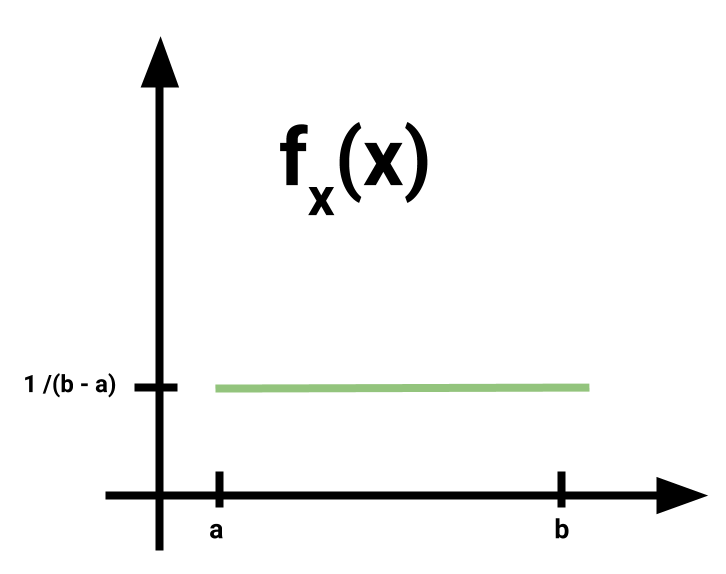
\includegraphics[width=0.45\textwidth]{UniformeContinua}
                \end{figure}










% //////////////////////////////////////////////////////////////////////////////////////////////////////////
% ////////////////////////////              FORMULARIO             /////////////////////////////////////////
% //////////////////////////////////////////////////////////////////////////////////////////////////////////
\part{CheatSheet - Formulario}
\clearpage


    % ===============================================================================
    % ===============                FORMULARIO                ======================
    % ===============================================================================
    \chapter{CheatSheet - Formulario}


        % ==============================================================
        % ===========       TEORIA DE CONJUNTOS         ================
        % ==============================================================
        \clearpage
        \section{Teoría de Conjuntos}

            \begin{table}[ht]
                \begin{tabular}{|m{16em}|m{16em}|@{}m{0pt}@{}}
                    \hline
                    \large{Nombre}          & \large{Propiedad}                             &\\[2em]    \hline\hline

                    \multicolumn{3}{|c|}{Operaciones Básicas}                                \\         \hline
                    Complemento  & $A' = \Set{x \Such x \notin X}$                          &\\[1em]    \hline
                    Intersección & $A \cap B = \Set{x \Such x \in A \text{ y } x \in B}$    &\\[1em]    \hline
                    Unión        & $A \cup B = \Set{x \Such x \in A \text{ ó } x \in B}$    &\\[1em]    \hline\hline

                    \multicolumn{3}{|c|}{Leyes de Morgan}                                    \\         \hline
                    Morgan sobre Unión          & $(A \cup B)' = A' \cap B'$                &\\[1em]    \hline
                    Morgan sobre Intersección   & $(A \cap B)' = A' \cup B'$                &\\[1em]    \hline\hline

                    \multicolumn{3}{|c|}{Combinatoria}                                       \\         \hline
                    Complemento  & $A' = \Set{x \Such x \notin X}$                          &\\[1em]    \hline
                    Intersección & $A \cap B = \Set{x \Such x \in A \text{ y } x \in B}$    &\\[1em]    \hline
                    Unión        & $A \cup B = \Set{x \Such x \in A \text{ ó } x \in B}$    &\\[1em]    \hline\hline
                  
                \end{tabular}
            \end{table}



        % ==============================================================
        % ===============        FORMULAS         ======================
        % ==============================================================
        \clearpage
        \section{Combinatoria}

            \begin{itemize}
                \item 
                    Número de \textbf{permutaciones} de un conjunto de $n$ objetos
                    \begin{equation*}
                        n!
                    \end{equation*}

                \item
                    Número de \textbf{muestras ordenadas} de tamaño $r$
                    \textbf{con remplazo} de un conjunto de $n$ objetos
                    \begin{equation*}
                        n^r
                    \end{equation*}

                \item
                    Número de \textbf{muestras ordenadas} de tamaño $r$
                    \textbf{sin remplazo} de un conjunto de $n$ objetos
                    \begin{align*}
                        {}_nP_r
                            = \frac{n!}{(n - r)!}          
                            = (n)(n-1)(n-2)\dots(n-r+1) 
                    \end{align*}

                \item
                    Número de \textbf{muestras no ordenadas} de tamaño $r$
                    \textbf{sin remplazo} de un conjunto de $n$ objetos

                    Esto es lo mismo que el número de subconjuntos de cardinalidad $r$ de
                    un conjunto de $n$ elementos
                    \begin{align*}
                        {n \choose r}
                            = {}_nC_r 
                            = \frac{{}_nP_r}{r!}          
                            = \frac{n!}{r!(n-r)!}          
                            = \frac{(n)(n-1)(n-2)\dots(n-r+1)}{r!}          
                    \end{align*}

                \item
                    Número de subconjuntos de un conjunto de $n$ elementos:
                    \begin{equation*}
                        2^n
                    \end{equation*}

                item
                    Las formas de permutar n elementos en un círculo es:
                    \begin{equation*}
                        (n - 1)!
                    \end{equation*}


            \end{itemize}


            % ==============================================================
            % ===============        FORMULAS         ======================
            % ==============================================================
            \clearpage
            \subsection{Propiedades Coheficientes Binomiales}

                \begin{itemize}

                    \item 
                        Propiedades Simetrícas
                        \begin{equation*}
                            {n \choose k} = {n \choose n - k}
                        \end{equation*}

                    \item 
                        Casos Especiales
                        \begin{align*}
                            {n \choose 0} = {n \choose n} = 1
                            \MegaSpace \MegaSpace
                            {n \choose 1} = {n \choose n-1} = n   
                        \end{align*}

                    \item 
                        Teorema del Binomio
                        \begin{equation*}
                            (x + y)^n 
                                = \sum_{k=0}^n {n \choose k} x^k y^{n-k}
                        \end{equation*}


                    \item 
                        Teorema del Binomio (Caso Especial)
                        \begin{equation*}
                            \sum_{k=0}^n {n \choose k} p^k (1 - p)^{n-k} = 1
                        \end{equation*}

                \end{itemize}



        % ==============================================================
        % =============       PROBABILIDAD        ======================
        % ==============================================================
        \clearpage
        \section{Probabilidad Básica}

            Definimos la probabilidad de un evento $A$ como:
            \begin{equation*}
                P(A) = \frac{|A|}{|S|} \Remember{Recuerda que $A$ es un evento y $S$ es espacio muestral}
            \end{equation*}

            % ====================================
            % =======    PROPIEDADES     =========
            % ====================================
            \subsection{Propiedades}

                \begin{itemize}
                    \item
                        $P(S) = 1$
                    
                    \item
                        Si $A_1, A_2, \dots, A_n$ son eventos mutuamente excluyentes entonces:
                        \begin{equation*}
                            P\Wrap{\bigcup_{i = 1}^n A_i} 
                                = \sum_{i = 1}^n P(A_i)    
                        \end{equation*}
                    
                    \item 
                        $P(\emptyset) = 0$
                    
                    \item 
                        $P(A') = 1 - P(A)$

                    \item 
                        Si $A \subseteq B$ entonces $P(A) \leq P(B)$

                    \item
                        La probabilidad de la unión de n eventos de puede escribir de manera general como:
                        \begin{equation*}
                            P\Wrap{\bigcup_{i = 1}^n A_i} 
                            = 
                                \sum_{i = 1}^n P(A_i) 
                                - \sum_{i < j}^n P(A_iA_j) 
                                + \sum_{i < j < k}^n P(A_iA_jA_k)
                                + \dots
                                + (-1)^{n+1} P\Wrap{\bigcap_{i = 1}^n A_i}
                        \end{equation*}
                    
                    \item Por consecuencia del caso general tenemos que: 
                        \begin{equation*}
                            P(A \cup B) = P(A) + P(B) - P(A \cap B)   
                        \end{equation*}
                    
                    \item Por consecuencia del caso general tenemos que: 
                        \begin{align*}
                            P(A \cup B \cup C) 
                                &=                                              \\
                                &P(A) + P(B) + P(C)                             \\
                                &-(P(A \cap B) + P(A \cap C) + P(B \cap C))     \\
                                &+ P(A \cap B \cap C)   
                        \end{align*}

                    \item
                        $P(A - B) = P(A) - P(A \cap B)$

                \end{itemize}


        % ==============================================================
        % ==================        PROBABILIDAD       =================
        % ==============================================================
        \clearpage
        \section{Probabilidad Condicional}

            La probabilidad de que ocurra el Evento $A$ conociendo que ya paso
            el Evento $B$ se denota y define como:
            \begin{equation*}
                P \Wrap{ A \Such B}
                    := \frac{P(A \cap B)}{P(B)}
                    = \frac{\Mag{A \cap B}}{\Mag{B}}
            \end{equation*}

            % ==============================================================
            % ============           PROPIEDADES           =================
            % ==============================================================
            \subsection{Propiedades}

                \begin{itemize}

                    \item
                        \textbf{Conservamos Propiedades}

                        La propiedad condicional cumple las propiedades que ya vimos de una propiedad
                        de un evento cualquiera, pero ahora el espacio muestral que antes era $S$ se
                        ha reducido.

                        \begin{itemize}
                            \item $P\Wrap{ A \Such B} + P\Wrap{ A' \Such B} = 1$
                            \item $P\Wrap{ A \cup B \Such C} 
                                        = P\Wrap{A \Such C} + P\Wrap{B \Such C}
                                        - P\Wrap{A \cap B \Such C}$
                        \end{itemize}


                    \item
                        \textbf{Definición Alterna}

                        Podemos redefinir a la probabilidad condicional como: 
                        $P \Wrap{ A \Such B} = \dfrac{\Mag{A \cap B}}{\Mag{B}}$

                    \item 
                        \textbf{Regla de Multiplicación}

                        Podemos escribir a $P(A \cap B)$ en terminos de probabilidad condicional.
                        \begin{equation*}
                            P(A \cap B)
                            = P(A | B) \; P(B)          
                            = P(B | A) \; P(A) 
                        \end{equation*}

                \end{itemize}

                    

        % ==============================================================
        % ===========      EVENTOS INDEPENDIENTES       ================
        % ==============================================================
        \clearpage
        \section{Eventos Independientes}

            Dados 2 eventos que $A, B$ son Independientes si y solo si
            $P(A) = P(A | B)$ y se escribe: $A \bot B$.


            % ==============================================================
            % ===========               PROPIEDADES         ================
            % ==============================================================
            \subsection{Propiedades}

                \begin{itemize}
                   
                    \item
                        Si $A \bot B$ entonces $P(A \cap B) = P(A) P(B)$
                        
                    \item
                        Si $A \bot B$ entonces $A' \bot B'$

                    \item
                        Si $A \bot B$ entonces $P(A \cap B) \neq 0$

                    \item
                        Si $P(A \cap B) = 0$ entonces $A, B$ no son eventos independientes

                \end{itemize}




            % ==============================================================
            % ===========      TEOREMA DE BAYES             ================
            % ==============================================================
            \subsection{Teorema de Bayes}

                Considera un conjunto de eventos $\Set{A_1, \dots, A_n}$ mutuamente excluyentes
                y tales que $\displaystyle \bigcup_{i=1}^n A_i = S$, es decir son particiones de $S$.

                Entonces podemos escribir la propabilidad de un evento $B$ donde $B \subset S$ como:
                \begin{equation*}
                    P(B) 
                        = \sum_{i = 1}^n P(B | A_i) \; P(A_i) 
                \end{equation*}


                Gracias a esto podemos decir que:
                \begin{align*}
                    P(A_i | B) 
                        = \frac{P(A_i \cap B)}{P(B)}                                                        \\
                        = \dfrac{P(B | A_i) \; P(A_i)}{\displaystyle \sum_{i = 1}^n P(A_i) \; P(B | A_i)}
                \end{align*}




        % ==============================================================
        % =======     VARIABLES ALEATORIAS DISCRETAS       =============
        % ==============================================================
        \clearpage
        \section{Variables Aleatorias Discretas}


            % ==============================================================
            % ===========      FUNCION PROBABILIDAD         ================
            % ==============================================================
            \subsection{Función Probabilidad $f_X$}


                % ======================================================
                % =======              PROPIEDADES      ================
                % ======================================================
                \subsubsection{Propieadades}

                    Es una función de probabilidad, es decir tiene que cumplir que la suma de todos los posibles
                    valores de la variable aleatoria den uno.

                    Más formalmente tenemos que la función probabilidad es aquella función que cumple que:
                    \begin{itemize}
                        \item $\forall a \in \Reals \MegaSpace 0 \leq f_X(a) \leq 1$
                        \item $\Set{x \Such f_X(x) \neq 0}$ es un conjunto finito o numerable
                        \item $\displaystyle \sum_x f_X(x) = 1$
                    \end{itemize}


            % ==============================================================
            % ===========      FUNCION ACUMULADA            ================
            % ==============================================================
            \clearpage
            \subsection{Función P. Acumulada $F_X$}

                % ======================================================
                % ===========          DEFINICIÓN       ================
                % ======================================================
                \subsubsection{Definición}

                    Describimos a la función de probabilidad acumulada como:
                    \begin{equation*}
                        F_X(x) = \sum_{i \leq x} f_{X}(i)
                    \end{equation*}

                % ======================================================
                % ===========          PROPIEADES       ================
                % ======================================================
                \subsubsection{Propiedades}

                    \begin{itemize}
                        \item
                            Una característica muy común es que:
                            \begin{itemize}
                                \item $\lim_{x \to -\infty} F_X (x) = 0$
                                \item $\lim_{x \to \infty} F_X (x) = 1$
                            \end{itemize}
                        \item
                            Si $x_1 \leq x_2$ entonces $F_X(x_1) \leq F_X(x_2)$
                    \end{itemize}



                % ======================================================
                % =======     FUNCION FUNDAMENTAL       ================
                % ======================================================
                \subsubsection{Función Fundametal}

                    Podemos ver a la acumulada como una función fundamental, tal que
                    podemos escribir a todas las demás:
                    \begin{itemize}
                        \item $P(X = x)             = F_X(x) - F_X(x - 1)$
                        \item $P(X < x)             = F_X(x - 1)$
                        \item $P(X \leq x)          = F_X(x)$
                        \item $P(X > x)             = 1 - F_X(x)$
                        \item $P(X \geq x)          = 1 - F_X(x - 1)$
                        \item $P(a \leq X \leq b)   = F_X(b) - F_X(a - 1)$
                        \item $P(a < X \leq b)      = F_X(b) - F_X(a)$
                        \item $P(a \leq X < b)      = F_X(b - 1) - F_X(a)$
                        \item $P(a < X < b)         = F_X(b - 1) - F_X(a - 1)$
                    \end{itemize}
                    


            % ==============================================================
            % ===========           ESPERANZA O MEDIA       ================
            % ==============================================================
            \clearpage
            \subsection{Esperanza o Media}

                % ======================================================
                % ===========          DEFINICIÓN       ================
                % ======================================================
                \subsubsection{Definición}

                    Decimos que el valor esperado, esperanza ó media de la variable $X$
                    se define como:
                    \begin{equation*}
                        \mu_{X} = E(X) = \sum_x \; x \; f_X(x) = \sum_x \; x \; P(X = x)
                    \end{equation*}

                % =========================================================
                % ===============        PROPIEDADES      =================
                % =========================================================
                \subsubsection{Propiedades}

                    \begin{itemize}

                        \item 
                            Si $X$ puede tomar un número infinito de valores entonces la esperanza de 
                            $X$ existe si y solo si $\displaystyle \sum_x |x| f_X(x) < \infty$

                        \item
                            Podemos dar una definición al evaular la esperanza sobre una función:
                            \begin{equation*}
                                E(g(x)) = \sum_x \; g(x) \; f_X(x)    
                            \end{equation*}

                        \item Es un Operador Lineal, es decir:
                            \begin{equation*}
                                E(\alpha X + \beta Y) = \alpha E(X) + \beta E(Y)   
                            \end{equation*}

                        \item
                            Si $X, Y$ son independientes entonces:
                            \begin{equation*}
                                E(XY) = E(X) E(Y)  
                            \end{equation*}

                        \item
                            Si $a$ es una constante, entonces: 
                            \begin{equation*}
                                E(a) = a
                            \end{equation*}

                    \end{itemize}


            % ==============================================================
            % ===========              VARIANZA             ================
            % ==============================================================
            \clearpage
            \subsection{Varianza}

                % ======================================================
                % ===========          DEFINICIÓN       ================
                % ======================================================
                \subsubsection{Definición}

                    Decimos que la varianza de la variable $X$
                    con $f_{X}(x)$ se define como:
                    \begin{equation*}
                        v(X) = E((X - \mu)^2)
                    \end{equation*}

   
                % ====================================================
                % ===========    DESVICACIÓN ESTANDAR       ==========
                % ====================================================
                \vspace{1em}
                \subsubsection{Desvianción Estandar}

                    Decimos que la desvianción estandar de la variable $X$
                    con $f_{X}(x)$ se define como:
                    \begin{equation*}
                        \sigma(X) = \sqrt{v(X)}
                    \end{equation*}

                    Se usa generalmente por las unidades que tiene la varianza, nada mas


                % ==============================================================
                % ===============        PROPIEDADES      ======================
                % ==============================================================
                \subsubsection{Propiedades}

                    \begin{itemize}

                        \item
                            $v(X) = E(X^2) - (E(X))^2$

                        \item 
                            $V(a) = 0$

                        \item 
                            $v(aX) = a^2 v(X)$


                        \item 
                            $v(X + Y) = v(X) + v(Y) + 2Cov(X,Y)$

                        \item 
                            $v(X - Y) = v(X) - v(Y) - 2Cov(X,Y)$
                                

                        \item
                            Si $X$ y $Y$ son independientes, entonces $v(X + Y) = v(X) + v(Y)$


                        \item
                            En general si $X_1, X_2, \dots, X_n$ son variables aleatorias, entonces
                            tenemos que:
                            \begin{align*}
                                v\Wrap{\sum_{i = 1}^n X_i} = \sum_{i = 1}^n X_i + 2\sum_{i < j}^n Cov(X_i, X_j)
                            \end{align*}

                    \end{itemize}
                                


            % ==============================================================
            % ===========            COVARIANZA             ================
            % ==============================================================
            \clearpage
            \subsection{Covarianza}

                % ======================================================
                % ===========          DEFINICIÓN       ================
                % ======================================================
                \subsubsection{Definición}

                    Sea $X, Y$ dos variables independientes, entonces
                    definimos a la covarianza como:
                    \begin{equation*}
                        Cov(X, Y)
                            = E\Wrap{(X - \mu_{X})(Y - \mu_{Y})}
                    \end{equation*}

                    Es una manera de medir la dispersión conjunta de ambas variables.



                
                % =====================================================
                % ===============        PROPIEDADES      =============
                % =====================================================
                \subsubsection{Propiedades}

                    \begin{itemize}

                        \item 
                            $Cov(X, Y) = E(X Y) - \mu_{X}\mu_{Y}$


                        \item La covarianza de 2 variables independientes es cero

                                
                    \end{itemize}




            % ==============================================================
            % ===========        MOMENTOS CENTRALES         ================
            % ==============================================================
            \clearpage
            \subsection{Momentos Centrales}

                Si $X$ es una variable aleatoria tal que $E(X) = \mu_x$ entonces tenemos que:
                \begin{itemize}
                    \item 
                        El k-ésimo momento central esta definida como:
                        \begin{equation}
                            \mu_k^c 
                                = E\Brackets{(X - \mu)^k}
                                = \sum_x (x - \mu)^k P(X = x)
                        \end{equation}

                    \item 
                        El k-ésimo momento alrededor del origen esta definida como:
                        \begin{equation}
                            \mu_k^0 
                                = E\Wrap{X^k}
                                = \sum_x x^k P(X = x)
                        \end{equation}

                \end{itemize}






                % ==============================================================
                % ===========     FUNCION GENERADORA      ======================
                % ==============================================================
                \clearpage
                \subsubsection{Función Generadora de Momentos}

                    La podemos definir como:
                    \begin{equation*}
                        \Psi_X (t) 
                            = E(e^{tX})
                            = \sum_x e^{tx} P(X = x)
                    \end{equation*}

                    Solemos decir que la k-ésima derivada de la función generadora
                    de momentos evaluada en $t = 0$ da como resultado el k-ésimo momento central al origen

                    Es decir, siguen el siguiente patrón:
                    \begin{itemize}
                        \item $\Psi_X' (t = 0) = E(X)$ 
                        \item $\Psi_X'' (t = 0) = E(X^2)$ 
                        \item $\Psi_X''' (t = 0) = E(X^3)$ 
                        \item $\Psi_X^{(n)} (t = 0) = E(X^n)$ 
                    \end{itemize}



                % ==============================================================
                % ===============        PROPIEDADES      ======================
                % ==============================================================
                \subsubsection{Propiedades}

                    \begin{itemize}

                        \item
                            Nota que $\Psi_x(a) = E(e^{aX})$

                        \item
                            Si $Y = aX + b$ entonces tenemos que:

                            $\Psi_Y(t) = e^{bt} \Psi_X(at)$


                        \item
                            $\Psi_X (t = 0) = \mu_k$

                        \item
                            $\Psi_X (t = 0) = E(X)$

                        \item
                            Nota que si tuvieramos un montón de variables aleatorias
                            $X_1, X_2, X_3, \dots, X_n$
                            Y decimos que $\displaystyle Y = \sum_{i = 1}^n X_i$

                            Entonces tenemos que:
                            \begin{equation*}
                                \Psi_Y(t) = \prod_{i = 1}^n \Psi_{X_i}(t)
                            \end{equation*}



                    \end{itemize}






% ===============================================
% ========        BIBLIO      ===================
% ===============================================
\begin{thebibliography}{10}

    \bibitem{Leticia} 
        Leticia Cañedo Suárez
        \textit{Probabilidad}. 
        ESCOM, 2018

\end{thebibliography}


\end{document}